\documentclass[a4paper,10pt]{article}
\usepackage{url}
\usepackage{hyperref}
\usepackage{fullpage}
\usepackage{booktabs}
\usepackage{graphicx}
\usepackage{wrapfig}
\usepackage{caption}
\usepackage{float}
\usepackage{subcaption}
\usepackage{enumerate}
\usepackage{color}
\usepackage{capt-of}
\usepackage{todonotes}
\usepackage{geometry}
 \geometry{
   a4paper,
   total={170mm,257mm},
   left=20mm,
   right=20mm,
   top=15mm,
 }
 \hypersetup{
    colorlinks=true,       % false: boxed links; true: colored links
    linkcolor=blue,        % color of internal links
    citecolor=blue,        % color of links to bibliography
    filecolor=magenta,     % color of file links
    urlcolor=blue
}
\usepackage{indentfirst}
  \setlength{\parindent}{0.5em}
  \setlength{\parskip}{0.1em}  
  % spacing: how to read {12pt plus 4pt minus 2pt}
%           12pt is what we would like the spacing to be
%           plus 4pt means that TeX can stretch it by at most 4pt
%           minus 2pt means that TeX can shrink it by at most 2pt
%       This is one example of the concept of 'glue' in TeX
\usepackage{titlesec}
  \titlespacing\section{0pt}{0pt plus 4pt minus 2pt}{0pt plus 2pt minus 2pt}
  \titlespacing\subsection{0pt}{0pt plus 4pt minus 2pt}{0pt plus 2pt minus 2pt}
  \titlespacing\subsubsection{0pt}{0pt plus 4pt minus 2pt}{0pt plus 2pt minus 2pt}




\title{Applied Machine Learning\\Report on Practice Assignment}
\author{Team 34}
%\date{\today}
\date{Fall Semester 2017}
\begin{document}
\maketitle

\section{Introduction}

%When reporting on your work do not explain the techniques you are using. You do not have space for this. Focus on reporting only on the results you get when you apply these techniques. Do not forget that the report is 10 pages long maximum (single column, 10pt minimum) in PDF format. {\bf Pages beyond the tenth one will be ignored and material in these pages will not be graded.}

\section{Datasets}
%Describe here your dataset (dimension of data, number of images per class, number of classes, features representatives of each class). Add illustrative images of the elements in your dataset to help the reader understand what each class entails.

The initial dataset was composed of 4 classes with 12 images per class. Figure \ref{fig:class} shows the composition of the different classes, that were chosen based on their varied geometrical and chromatic features: Watches are dark and have a round shape, bananas are long and yellow, chairs have angular features and pens are long and thin. This representative features are summarized in Table \ref{tab::Dataset-characteristics}. 

\begin{figure}[H]
\centering
    \begin{subfigure}[t]{0.2\textwidth}
        \centering
        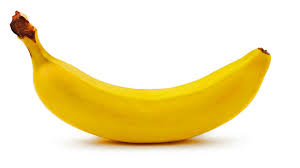
\includegraphics[height=2cm]{pictures/banana} 
        \caption{Banana}
        \label{fig:banana}
    \end{subfigure}%
    ~
    \begin{subfigure}[t]{0.2\textwidth}
        \centering
        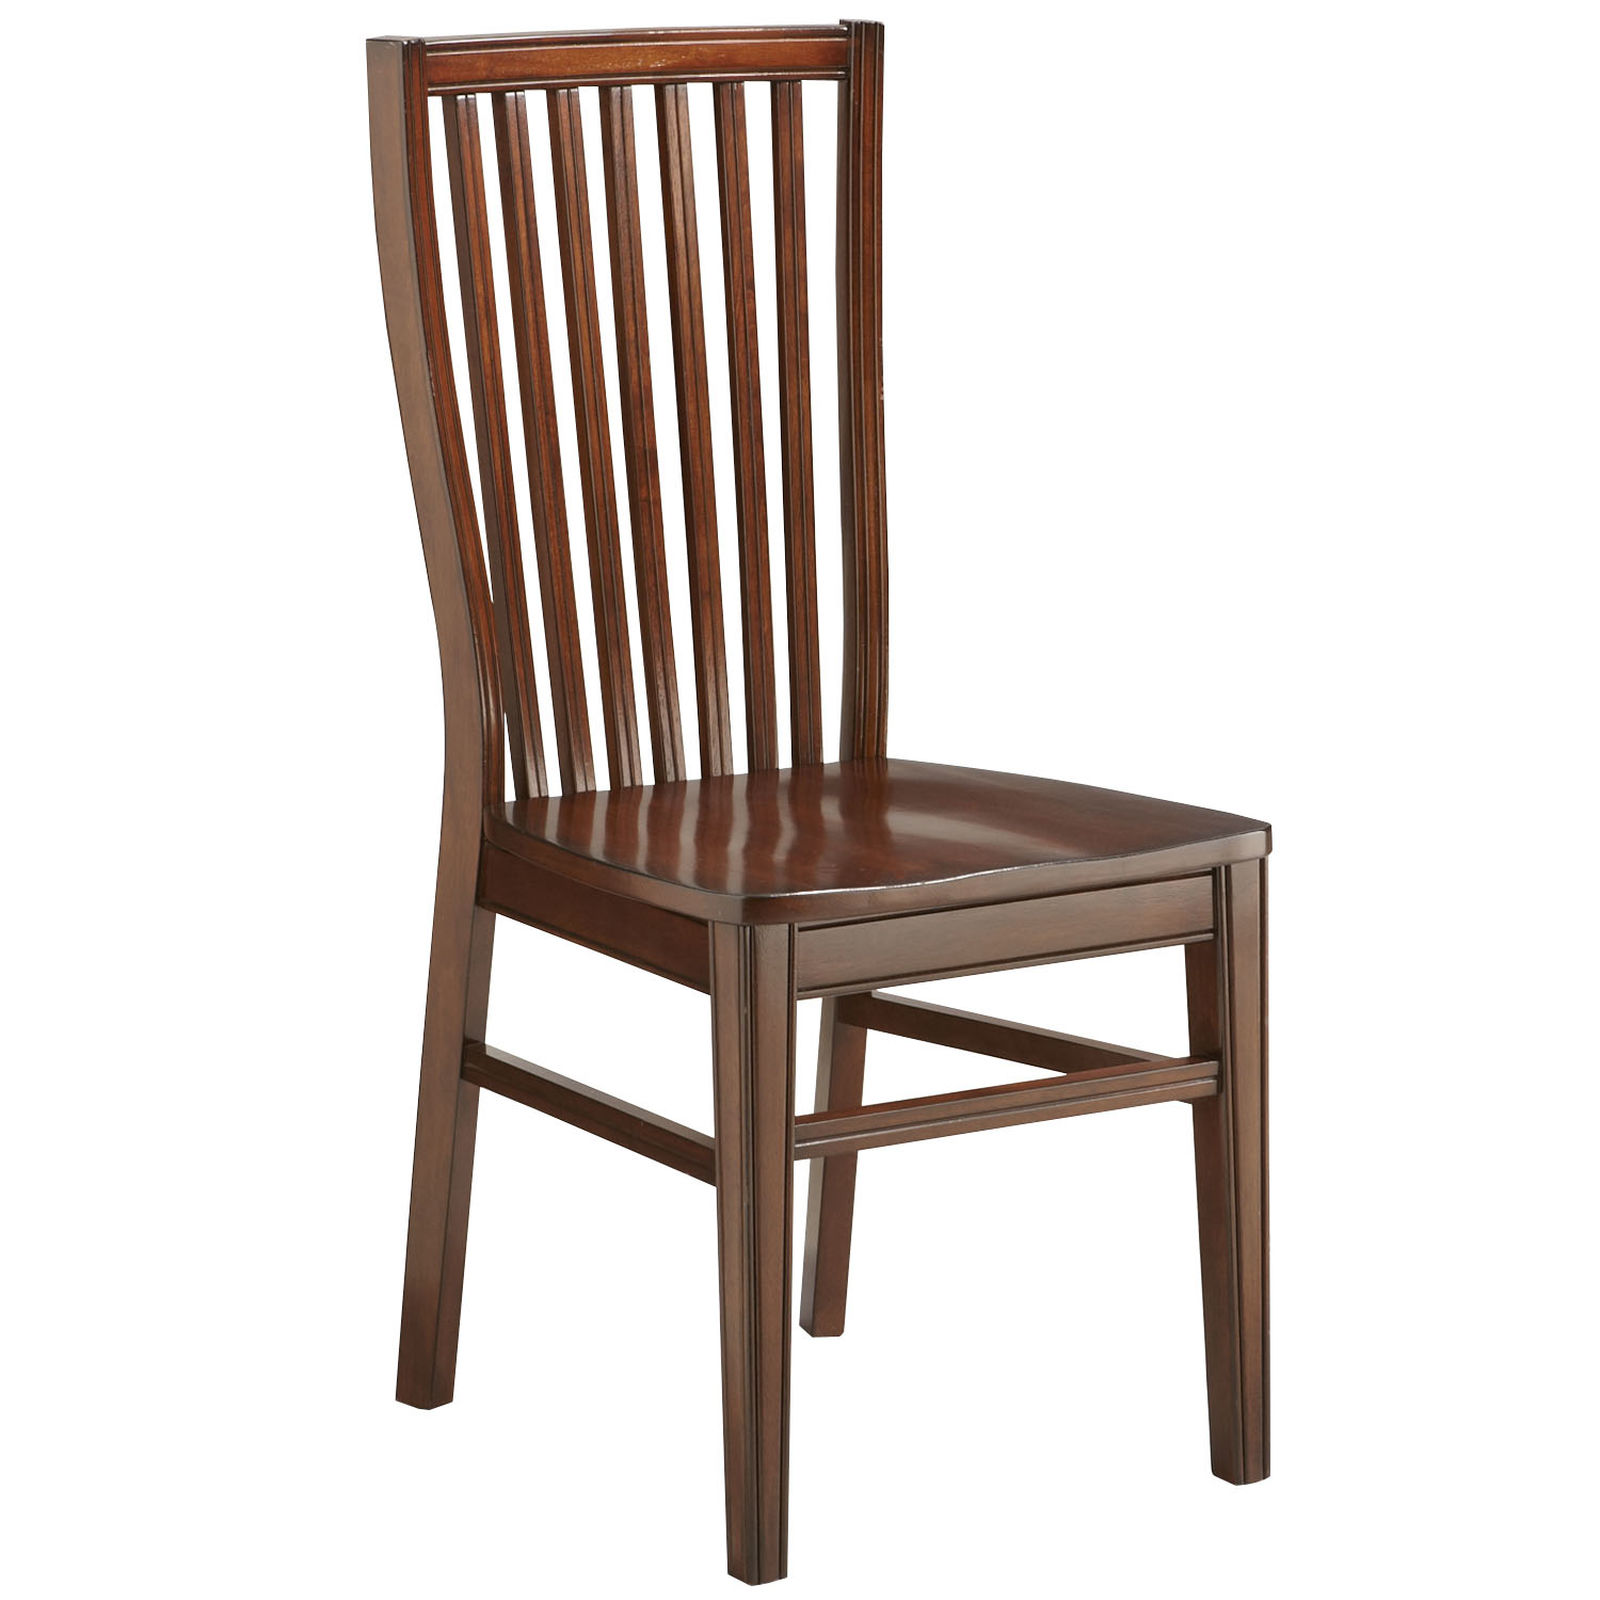
\includegraphics[height=2cm]{pictures/chair2} 
        \caption{Chair}
        \label{fig:chair}
    \end{subfigure} 
    ~
    \begin{subfigure}[t]{0.2\textwidth}
        \centering
        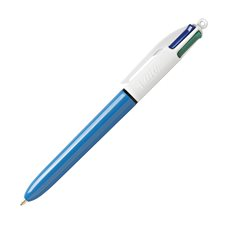
\includegraphics[height=2cm]{pictures/stylo4} 
        \caption{Pen}
        \label{fig:pen}
    \end{subfigure}
    ~
    \begin{subfigure}[t]{0.2\textwidth}
        \centering
        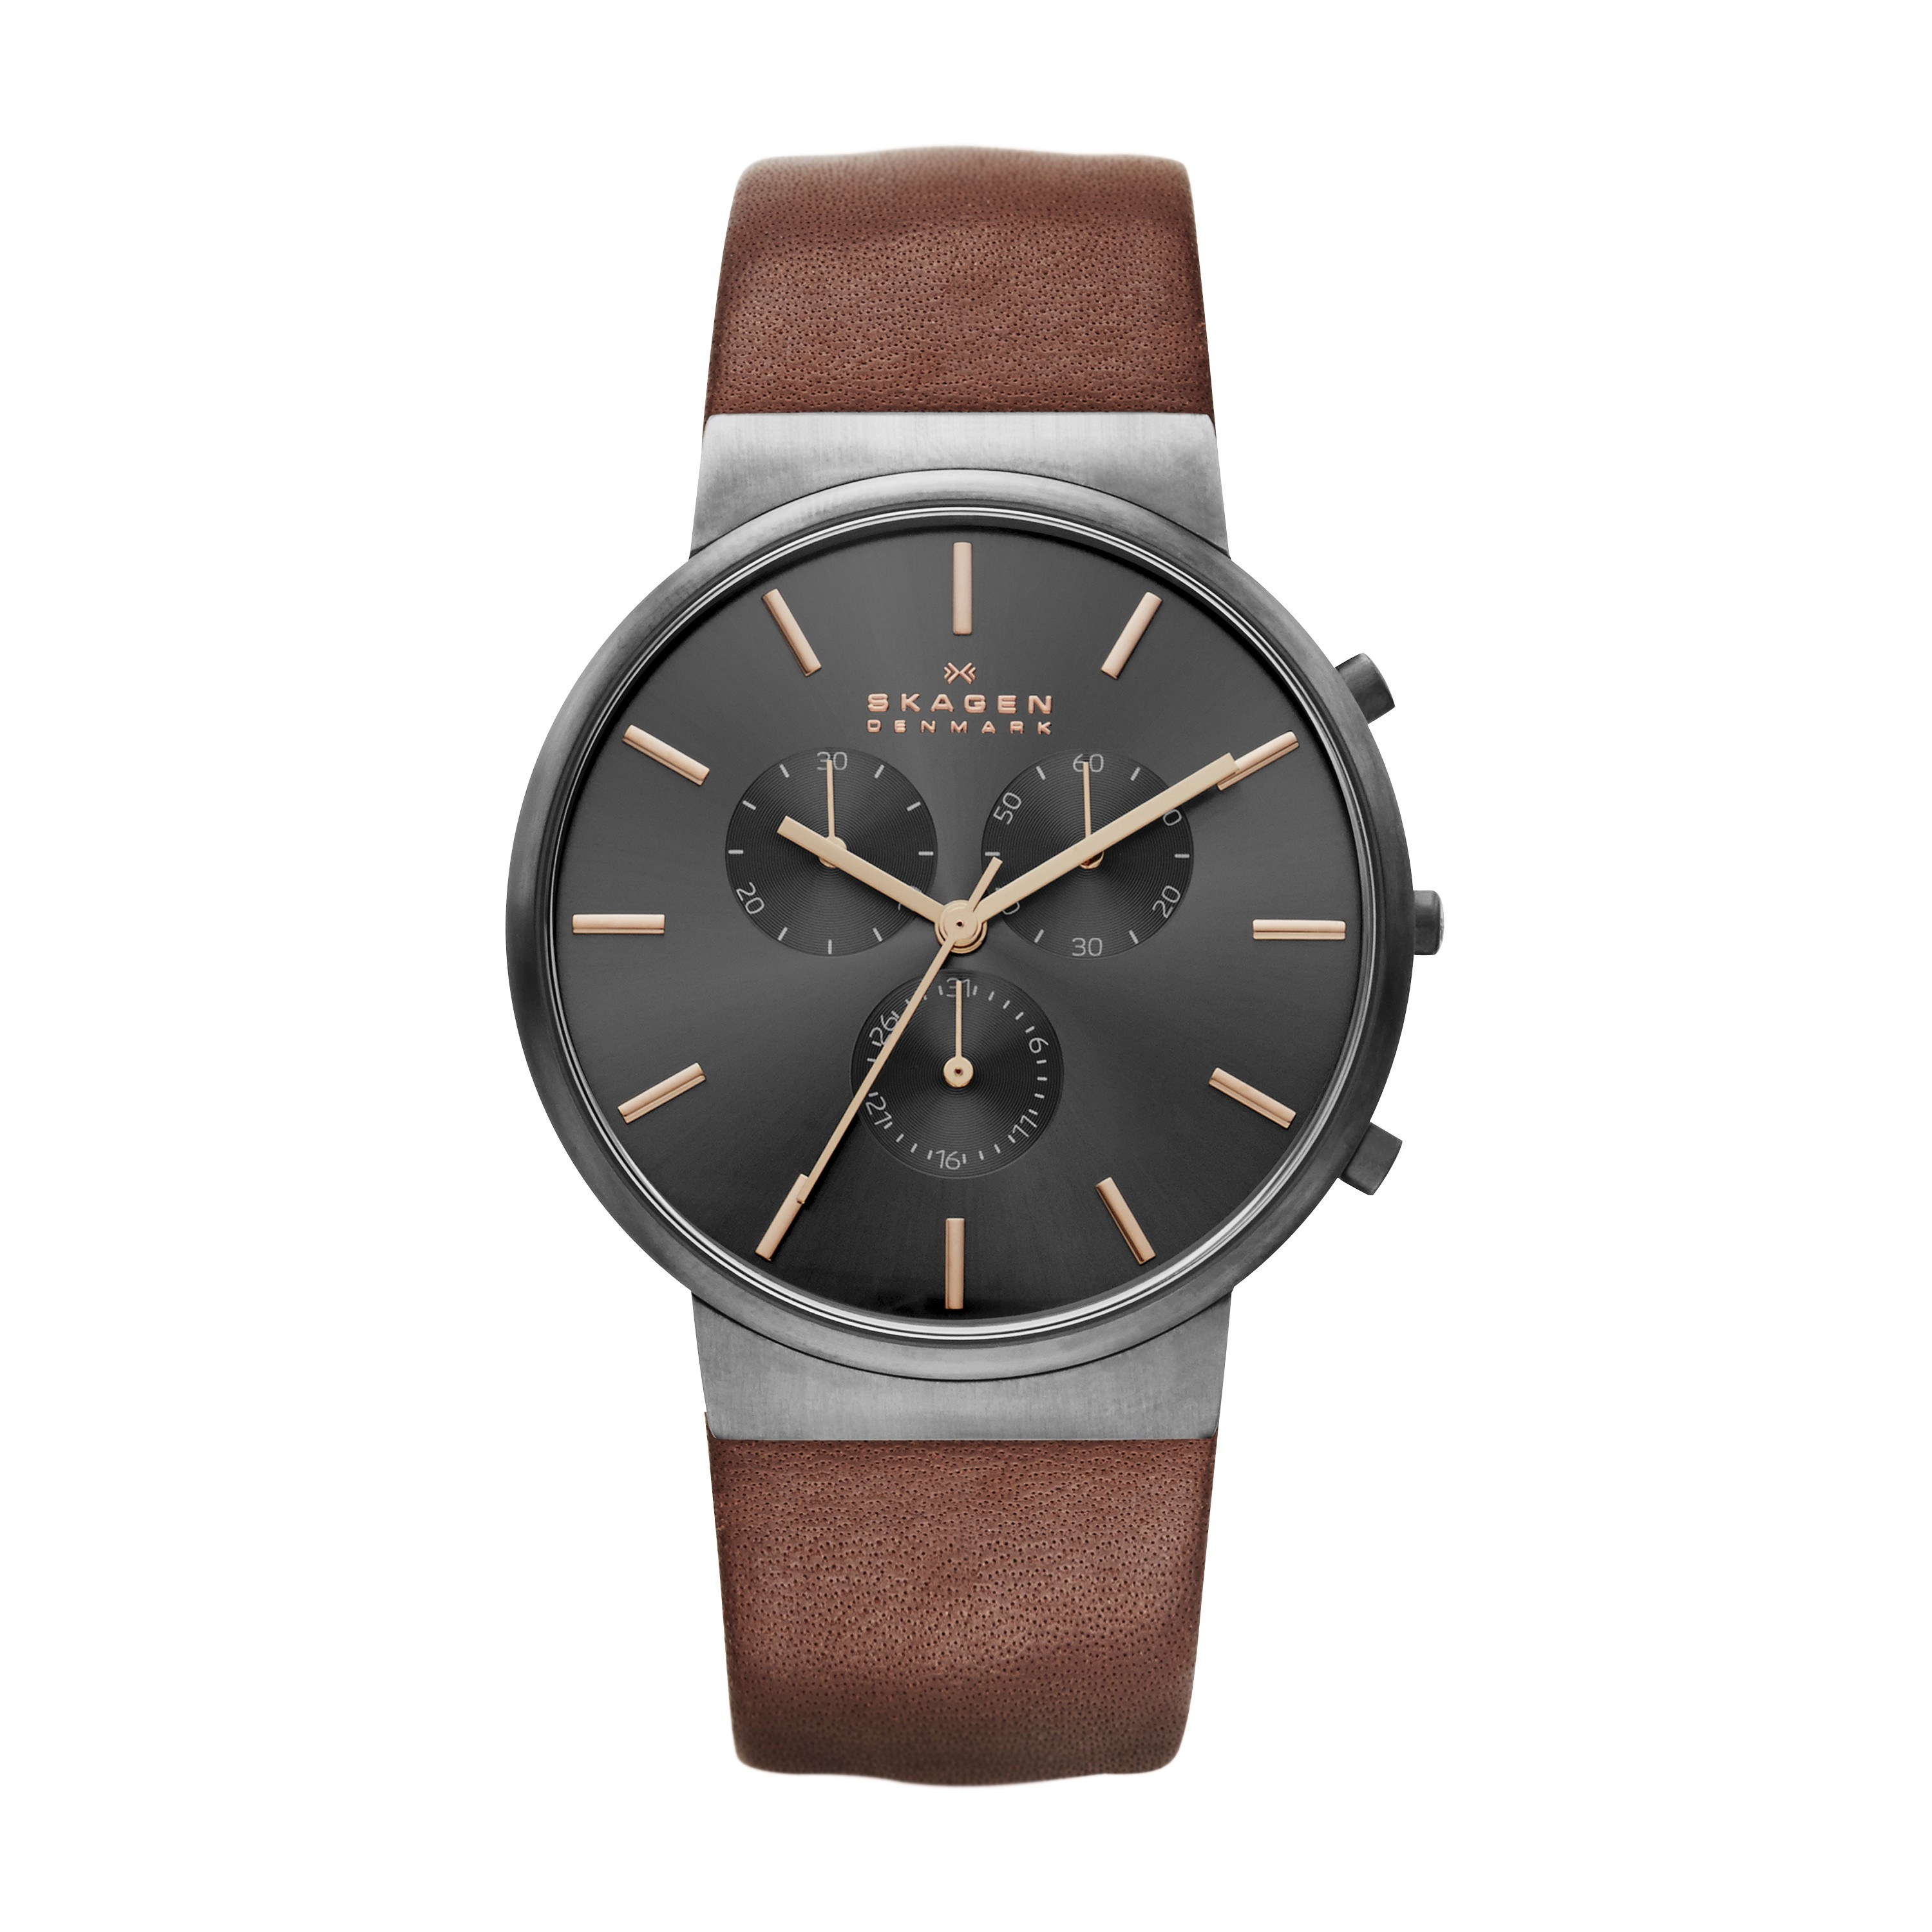
\includegraphics[height=2cm]{pictures/watch2} 
        \caption{Watch}
        \label{fig:watch}
    \end{subfigure}   
\caption{Four different classes}
\label{fig:class}
\end{figure}


The pictures are normalized when imported in MLDemos to have the same size. The initial dataset (see Figure \ref{fig:dataset_1}) is stored in a single $336 \times 336 $ image constituted of a 7 by 7 matrix of images. Thus, each image has a size of $48 \times 48$ pixels. With a RGB color format, there is and a number of features of $48\times48\times3$.


\begin{table}[H]
\centering
\begin{tabular}{|l|l|l|c|l|}
\hline
\textbf{Classes} & \textbf{Shape} & \textbf{Colour} & \multicolumn{1}{l|}{\textbf{\begin{tabular}[c]{@{}l@{}}Number \\ of images\end{tabular}}} & \textbf{\begin{tabular}[c]{@{}l@{}}Size\\ in pixels\end{tabular} } \\ \hline
Banana           & Long 			& Yellow         & 12                                                                                        & $48\cdot 48$                                                      \\ \hline
Pens             & Long and thin 	& Multicoloured  & 12                                                                                        & $48\cdot 48$                                                      \\ \hline
Watches          & Round 			& Dark          & 12                                                                                        & $48\cdot 48$                                                      \\ \hline
Chairs           & Angular			& Light        	& 12                                                                                        & $48\cdot 48$                                                      \\ \hline
\end{tabular}
\caption{Dataset characteristics}
\label{tab::Dataset-characteristics}
\end{table}

An effort was made to have a linear separable dataset in the beginning for learning purposes. In order to obtain that, the images for each class were purposely chosen to have similar caracteristics such as shape, color and orientation in space.
For the second part of this report the same dataset was used, but some noisy datapoints were added by hand in MLDemos (5 per class). This new dataset can be seen in Figure \ref{fig:dataset_new_2}. 

\begin{figure}[H]
\centering
	\begin{subfigure}[t]{0.3\textwidth}
      \centering
      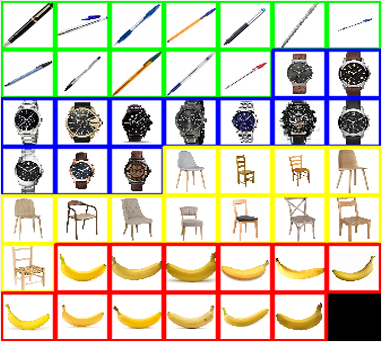
\includegraphics[width=0.8\textwidth]{pictures/dataset_1}
      \caption{Pictures in dataset 1}
      \label{fig:dataset_1}
    \end{subfigure}%
    ~
	\begin{subfigure}[t]{0.3\textwidth}
      \centering
      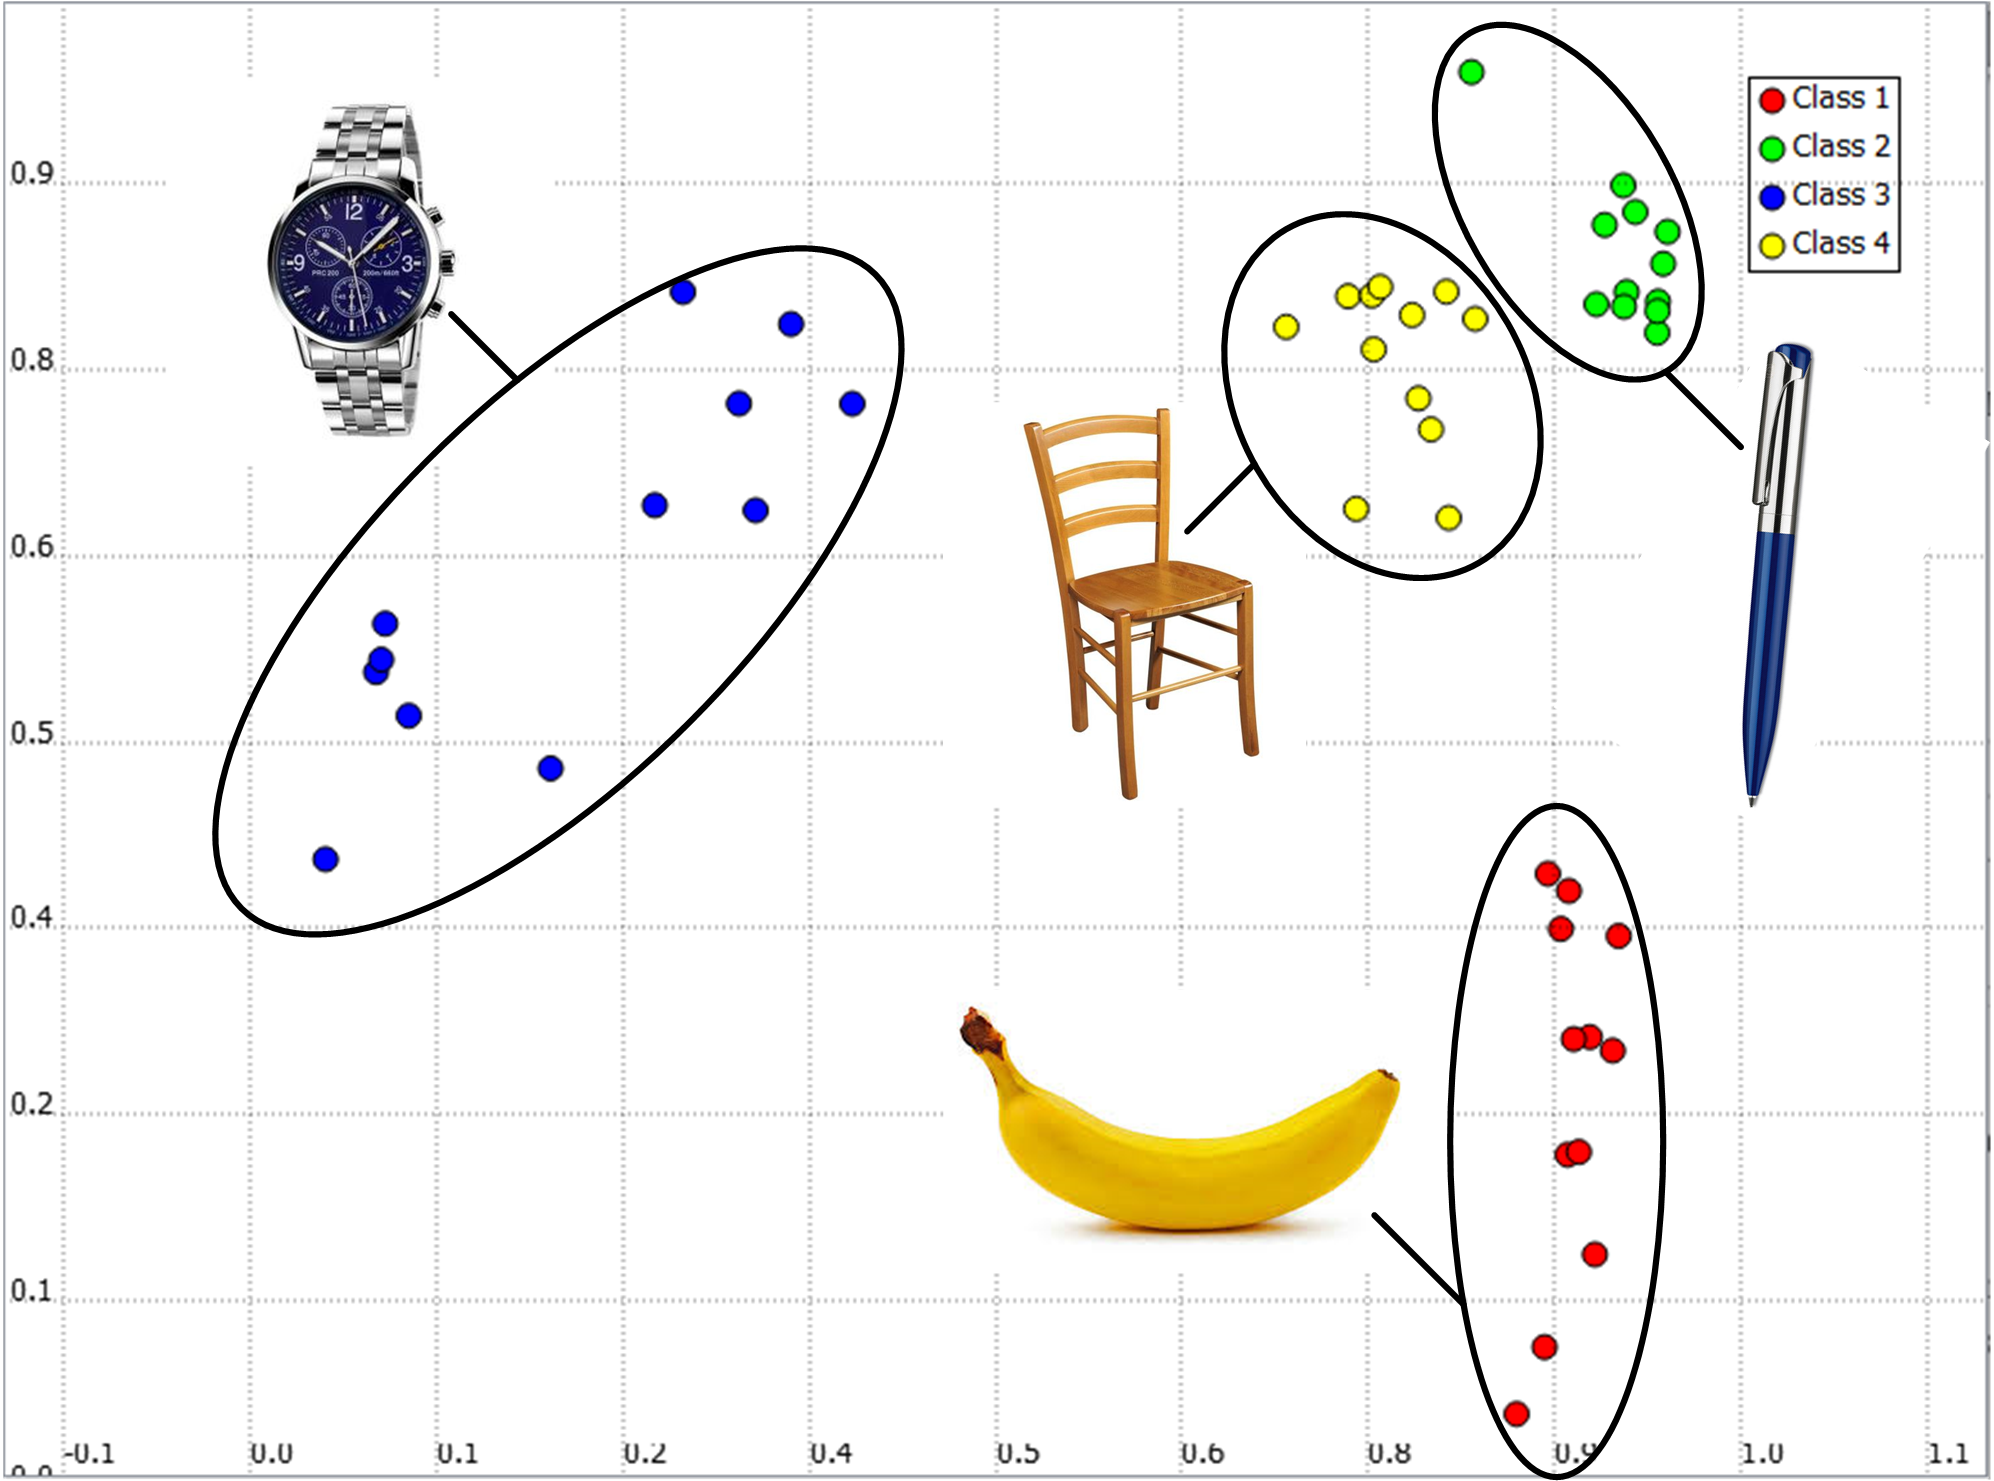
\includegraphics[width=\textwidth]{pictures/dataset_1_labelized}
      \caption{Projected datapoints of dataset 1}
      \label{fig:dataset_1_labelized}
    \end{subfigure}%
    ~
	\begin{subfigure}[t]{0.3\textwidth}
      \centering
      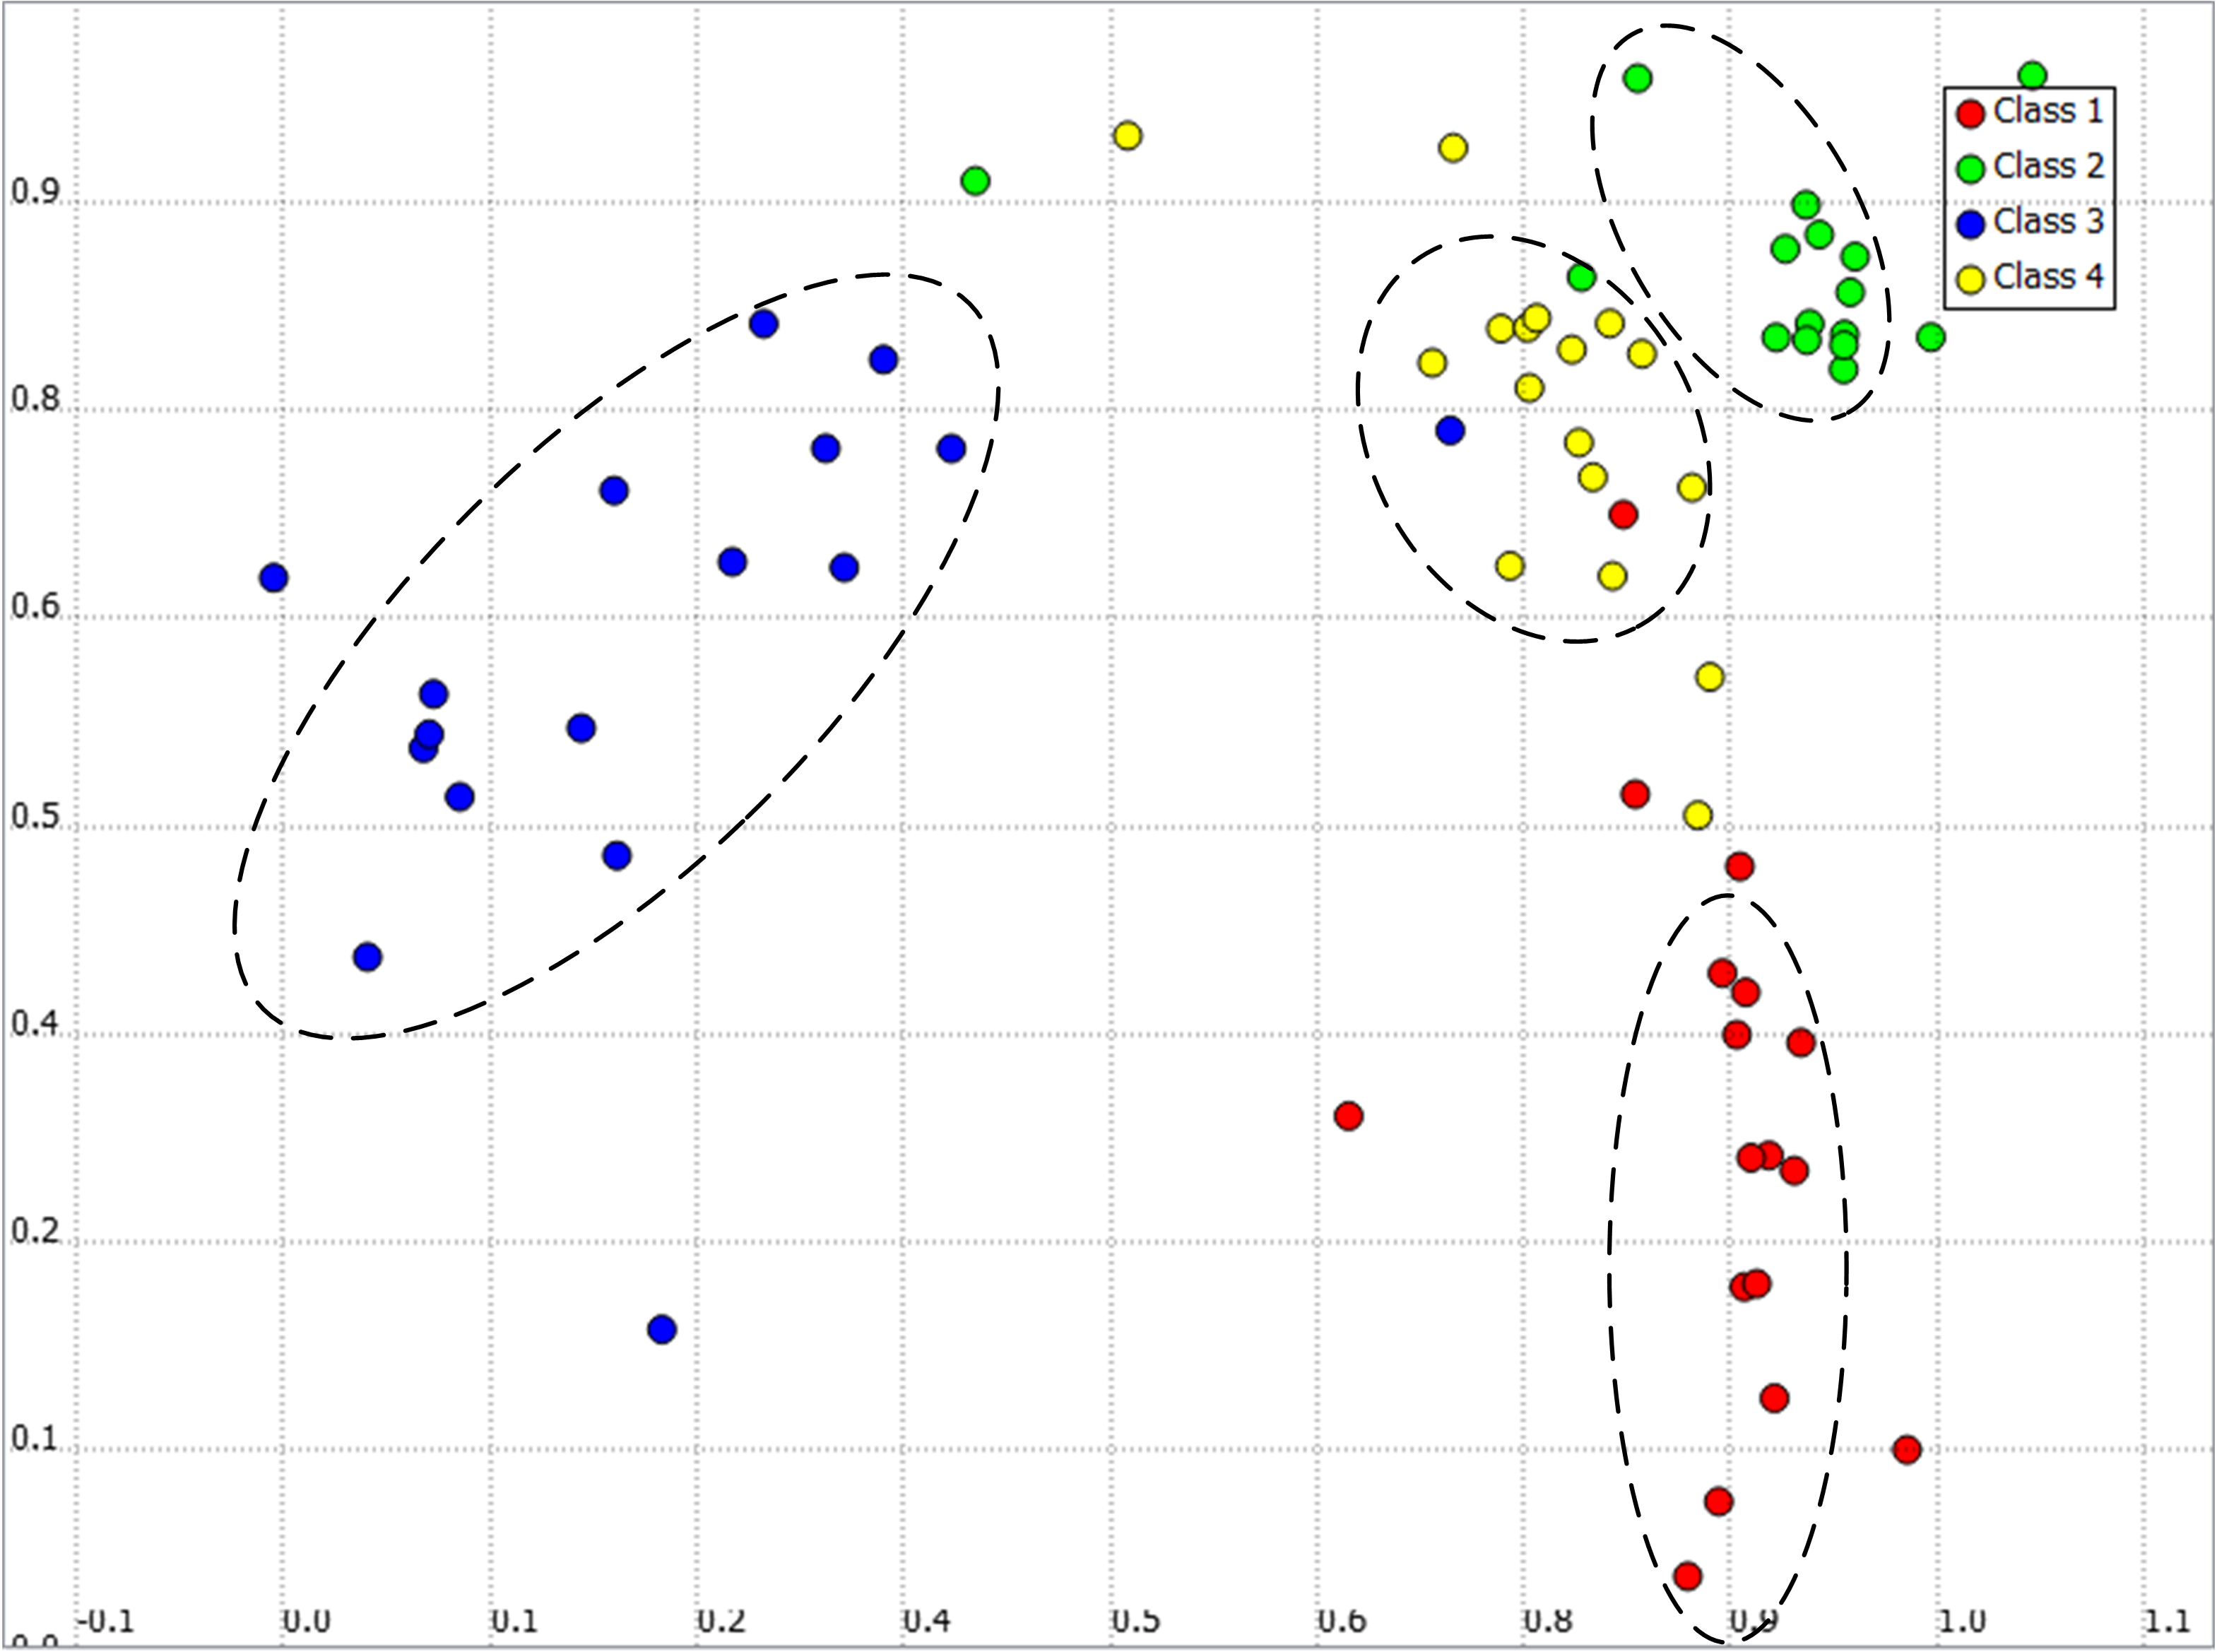
\includegraphics[width=\textwidth]{pictures/dataset_new_2}
      \caption{Projected datapoints of dataset 2}
      \label{fig:dataset_new_2}
    \end{subfigure}%
  \caption{Comparison of the datasets used for the report}
\end{figure}


\section{Dimensionality Reduction}
% Apply PCA on your dataset and choose the projections that allow you to best separate the classes. Expect to have to use several projections in combination to separate the classes. Keep these projections as you will use the data projected in these dimensions in the other practicals.


\begin{figure}[H]
\centering
     \begin{subfigure}[t]{0.3\textwidth}
      \centering
      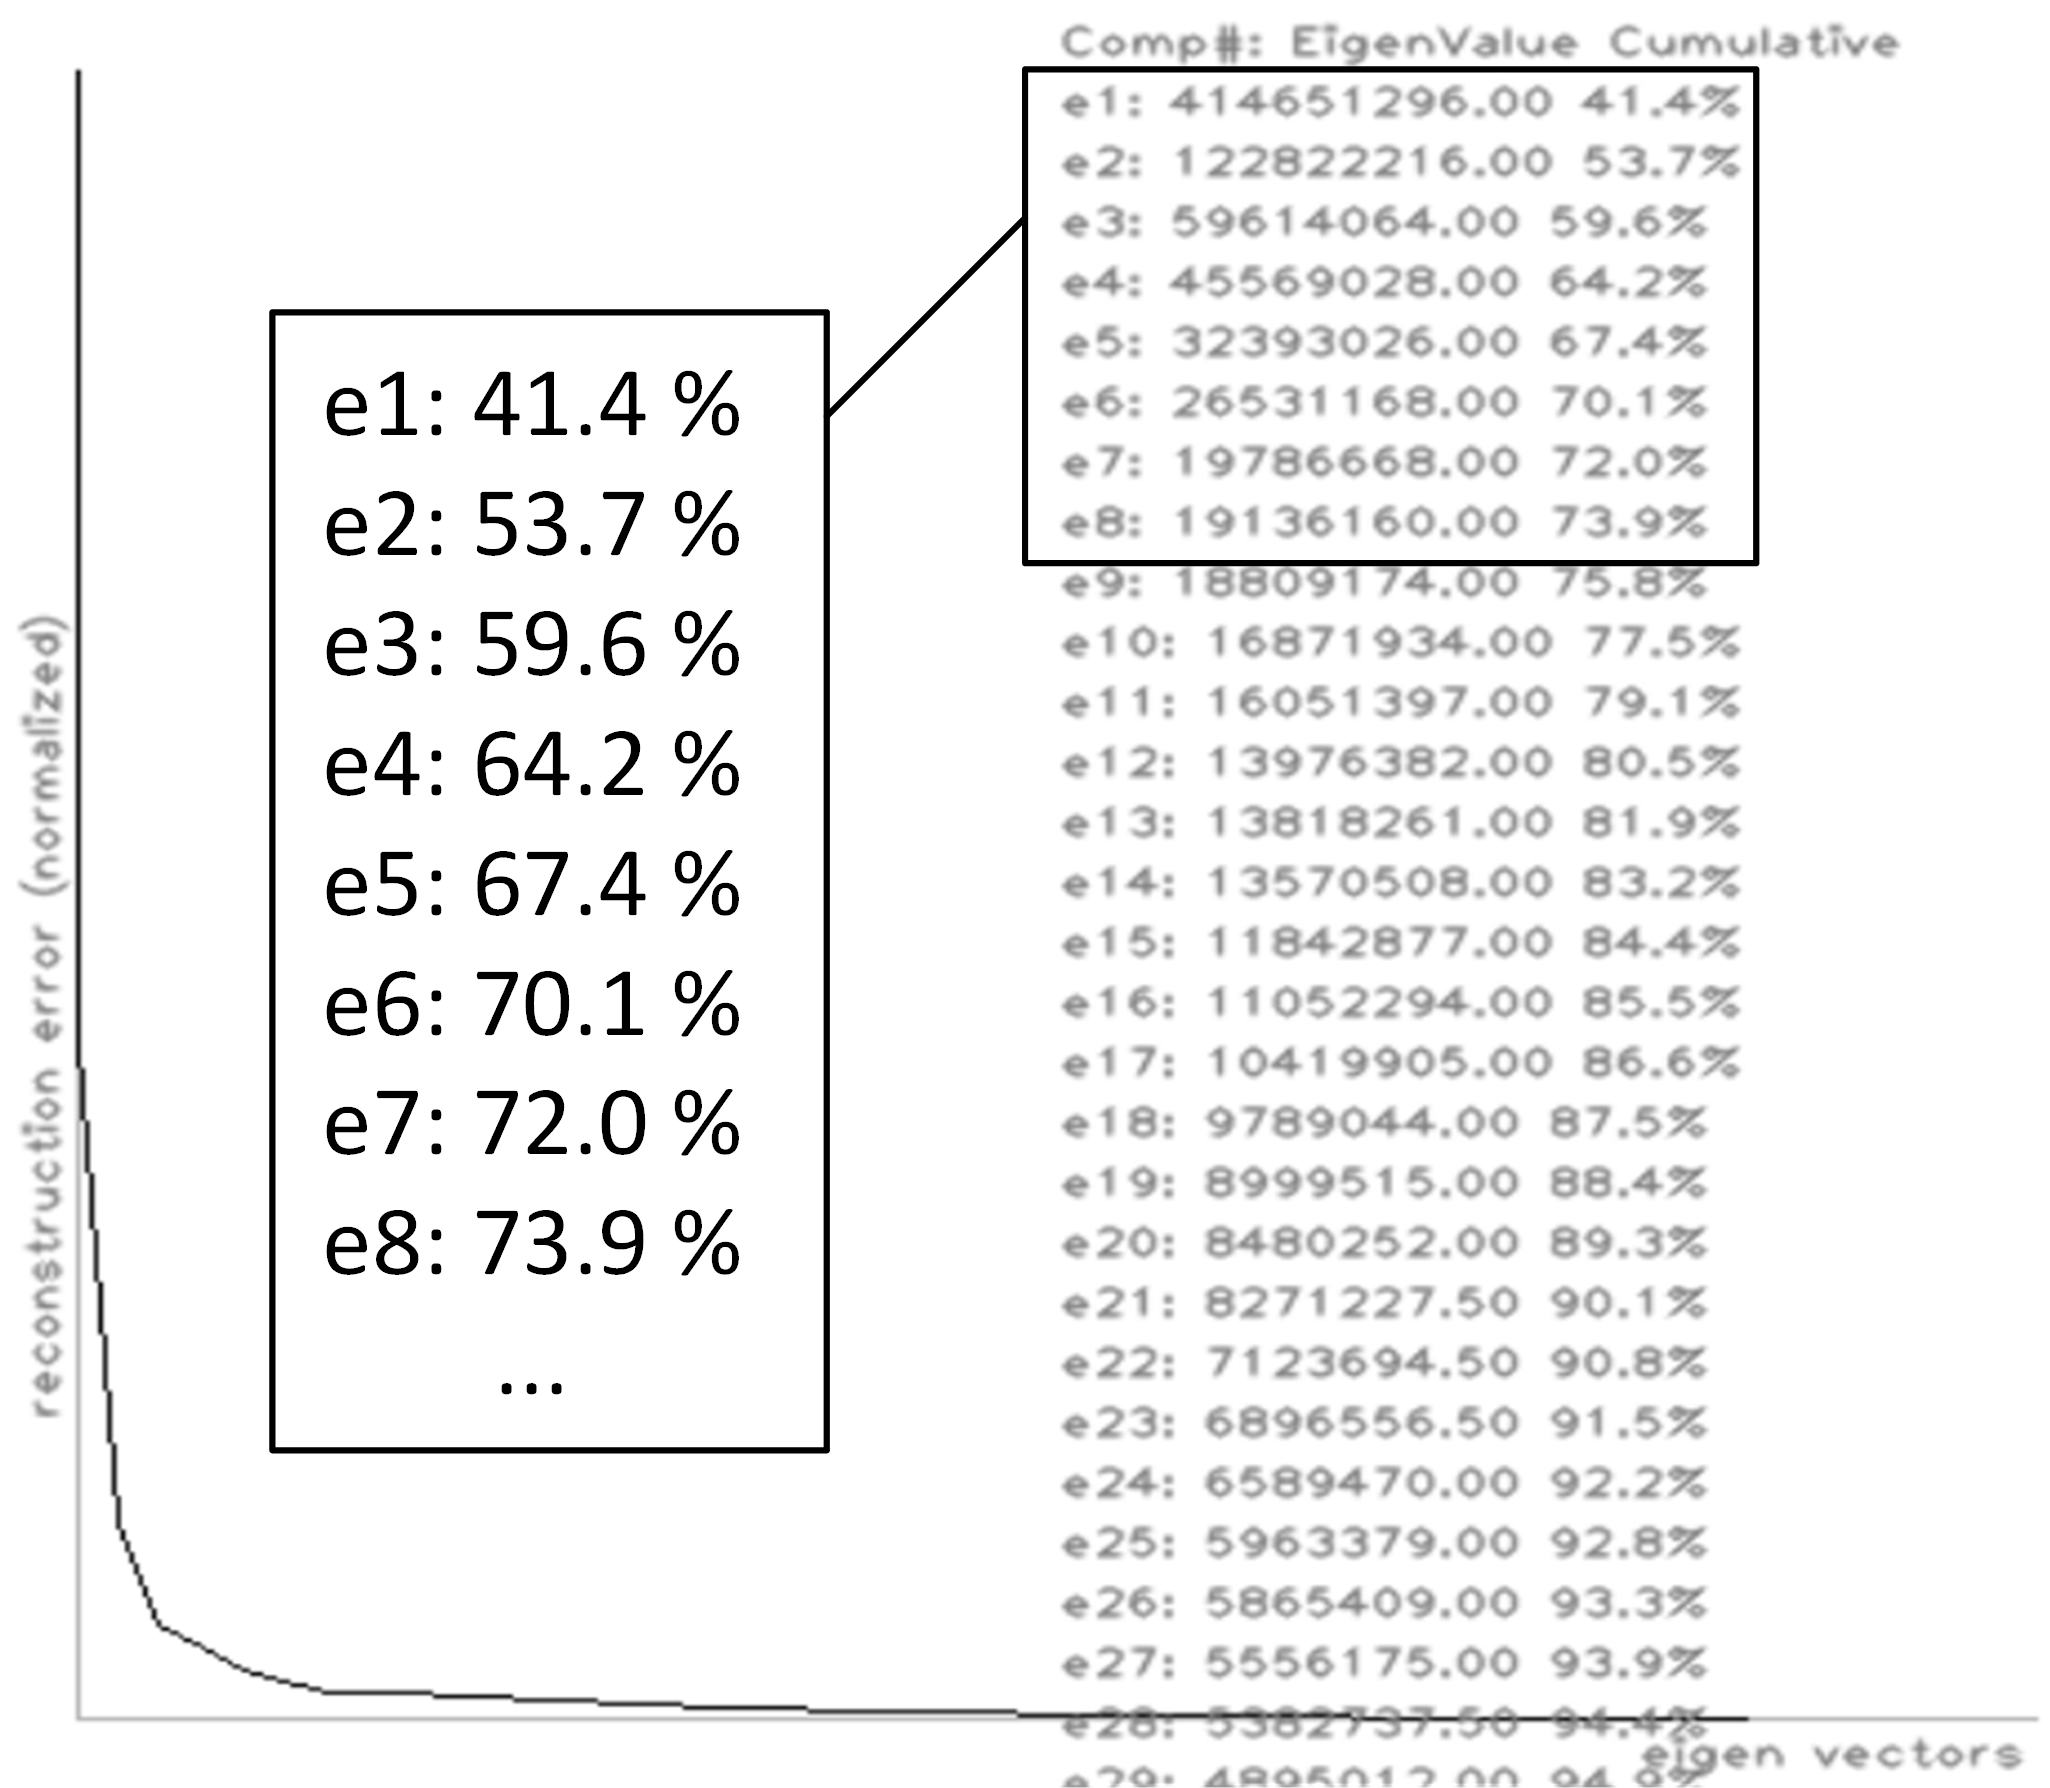
\includegraphics[width=0.8\textwidth]{pictures/eigenvalue_dataset1}
      \caption{Cumulative eigenvalues}
      \label{fig:eigenvalue_dataset1}
    \end{subfigure}%
    ~
    \begin{subfigure}[t]{0.3\textwidth}
      \centering
      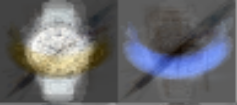
\includegraphics[width=\textwidth]{pictures/eigenvector_1}
      \caption{First two eigenvectors}
      \label{fig:eigenvector_1}
     \end{subfigure}
      ~
    \begin{subfigure}[t]{0.3\textwidth}
      \centering
      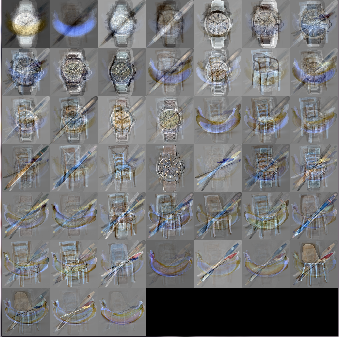
\includegraphics[width=4cm]{pictures/eigenvectors}
      \caption{All eigenvectors}
      \label{fig:eigenvectors}
     \end{subfigure}
     \caption{First PCA}
     \label{fig:PCA}
\end{figure}

\begin{figure}[H]
  \centering
  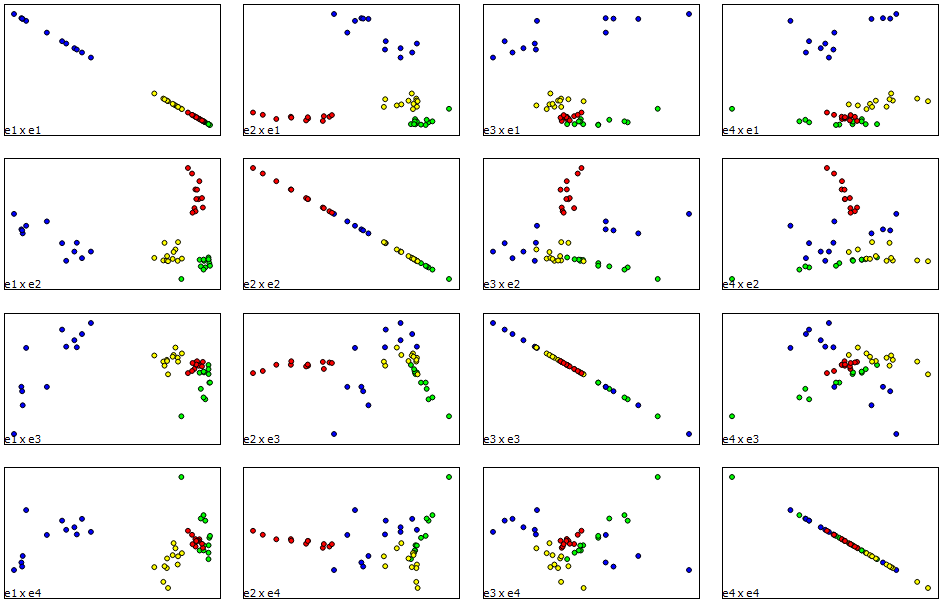
\includegraphics[height = 6cm]{pictures/PCA_projections}
  \caption{PCA projection matrix on eigenvectors 1 to 4}
  \label{fig:PCA_matrix}
\end{figure}

PCA was applied to the dataset 1. Figure \ref{fig:eigenvalue_dataset1} shows the cumulative reconstruction error: it can be noticed that 73.9\% of the dataset can be reconstructed with the first 8 eigenvectors. 
It can be seen in Figure \ref{fig:PCA_matrix} that the projection onto e1-e2 was the optimal projection for clustering purposes as expected: indeed they represent most of the variance of the data. The first eigenvector corresponds to a white watch, a yellow banana and the shape of a pen in the background. On the other hand the second eigenvector shows a blue banana, a pen and a shape of a chair in the background. As such, eigenvector 1 will separate well the watches class from the rest, while the second one will separate better the banana class from the rest. The two principal eigenvectors are shown in Figure \ref{fig:eigenvector_1} while the first 45 eigenvectors can be seen in Figure \ref{fig:eigenvectors}.
%It can be seen in Figure \ref{fig:eigenvector_1} that the first eigenvector has a strong correlation with the watches class while it is less predominant for the other classes. On the other hand, the second eigenvector has a strong correlation with the apple class and the shape of apples and watches influences the spreads of the two classes in a similar manner. Moreover, these classes are not linearly separable in the other projections (see Figure \ref{fig:PCA_matrix}).

\section{Clustering - qualitative assessment}
%   A qualitative assessment of the results from applying K-means, Soft K- Means, and DBSCAN in unsupervised mode to your dataset. A quantitative assessment of applying the same methods tested in semi-supervised clustering mode. Specifically, make sure to report i) the values tested for the hyperparameters of the clustering technique, and ii) the ratios across labelled and unlabelled points tested in semi-supervised mode.

% For K-means, try changing the type of metric (Euclidean, Manhattan, Infinite and Polynomial).
% Note : L1 bad for noise of class 2 (green)
% Test also the sensitivity to random initialization. 
% Note : all sensitive to initial position

In order to assess the functionalities of unsupervised clustering methods, the dataset 1 was used (see Figure \ref{fig:dataset_1}). In particular, the algorithms K-Means, Soft K-Means and DBScan were applied.

\subsection{K-means}

The hyperparameters for the K-means method are:
\begin{itemize}
\item the number of clusters;
\item the metric ($L_1$, $L_2$, $L_{\infty}$, $L_p$).
\end{itemize}

In Figure \ref{fig:good_kmeans}, correct results are shown for K-Means applied for K=4 and different metrics. It can be observed that the type of metric affects the shape of the borders between cluster. Indeed, $L_1$ defines distances that are the sum of the coordinates, as such the edges generated will have $n\cdot 45^{\circ}$ slopes. On the other hand, $L_2$ defines distances in the euclidian way, as such the edges generated will be straight. Finally, $L_p$ distances will generate higher parabolic functions, as the p degree of the polynomial function increases. When $p\rightarrow\infty$, $L_{\infty}$ is defined which generated the same edges as the $L_1$ metric. 

Although all metrics were able to correctly separate the classes, some errors were typically shown, as can be seen in Figure \ref{fig:bad_kmeans}. These errors can be mainly due to the random initialisation of K-Means (see Initialization below) and the fact that the classes do not have similar distributions, which is the condition K-Mean works best for. 

\begin{figure}[H]
\centering
    \begin{subfigure}[t]{0.2\textwidth}
      \centering
      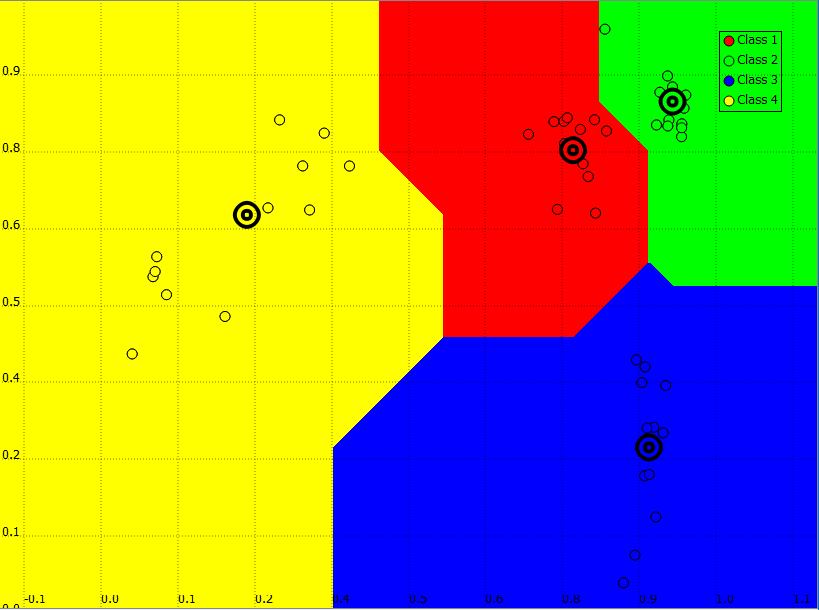
\includegraphics[width=\textwidth]{pictures/dataset_1_Kmeans-4K-L1}
      \caption{Metric L1}
      \label{fig:dataset_1_Kmeans-4K-L1}
     \end{subfigure}
      ~
    \begin{subfigure}[t]{0.2\textwidth}
      \centering
      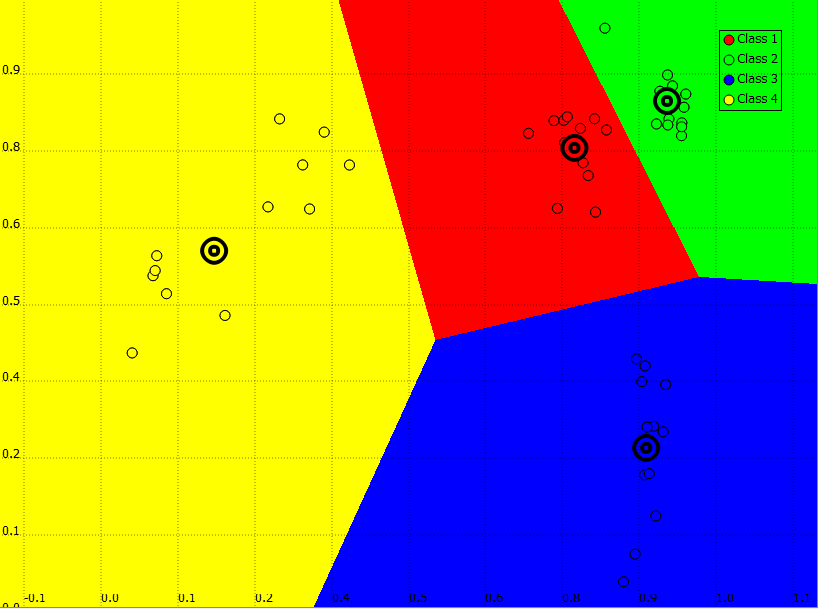
\includegraphics[width=\textwidth]{pictures/dataset_1_Kmeans-4K-L2}
      \caption{Metric L2}
      \label{fig:dataset_1_Kmeans-4K-L2}
     \end{subfigure}
      ~
    \begin{subfigure}[t]{0.2\textwidth}
      \centering
      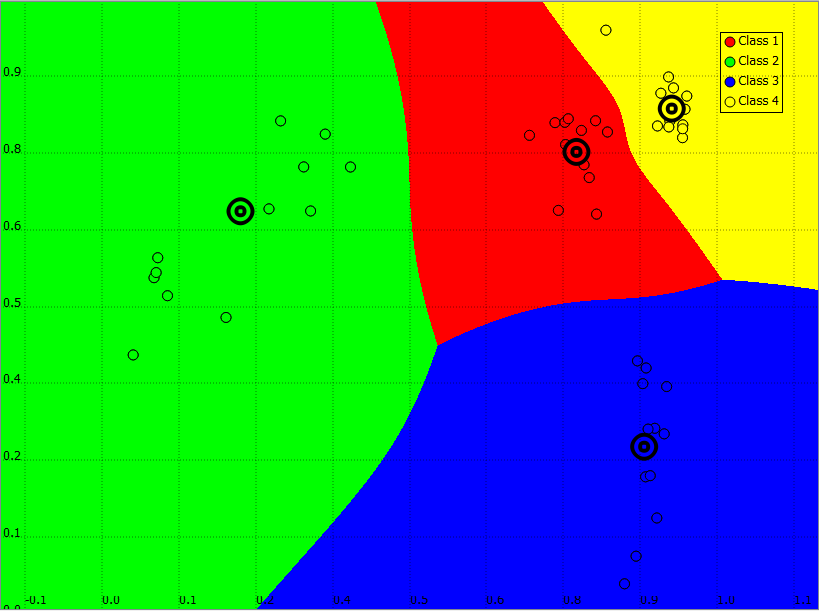
\includegraphics[width=\textwidth]{pictures/dataset_1_Kmeans-4K-L3}
      \caption{Metric Lp with p=3}
      \label{fig:dataset_1_Kmeans-4K-L3}
     \end{subfigure}
      ~
    \begin{subfigure}[t]{0.2\textwidth}
      \centering
      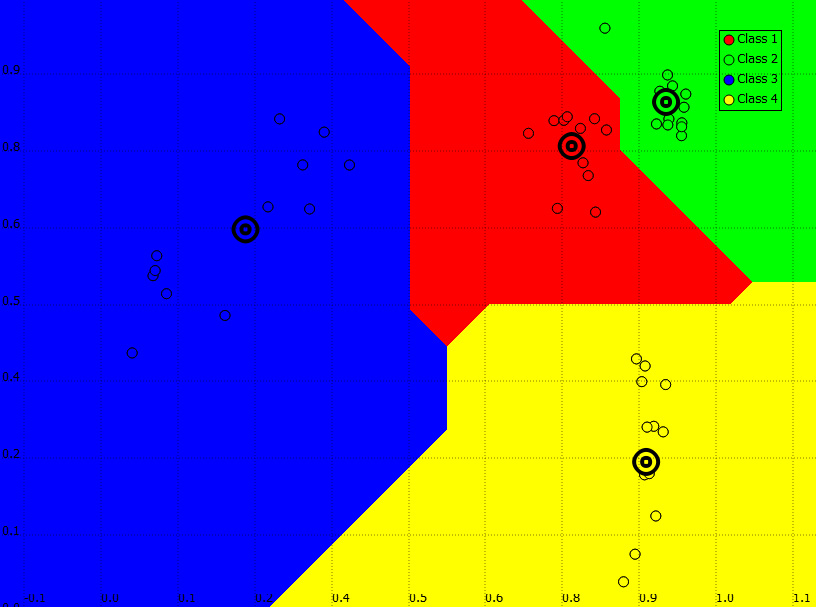
\includegraphics[width=\textwidth]{pictures/dataset_1_Kmeans-4K-Linf}
      \caption{Metric Linf}
      \label{fig:dataset_1_Kmeans-4K-Linf}
     \end{subfigure}
     \caption{Dataset 1 with correct K-Means clustering, different metrics and K=4}
     \label{fig:good_kmeans}
\end{figure}



%Bad results
\begin{figure}[H]
\centering
    \begin{subfigure}[t]{0.2\textwidth}
      \centering
      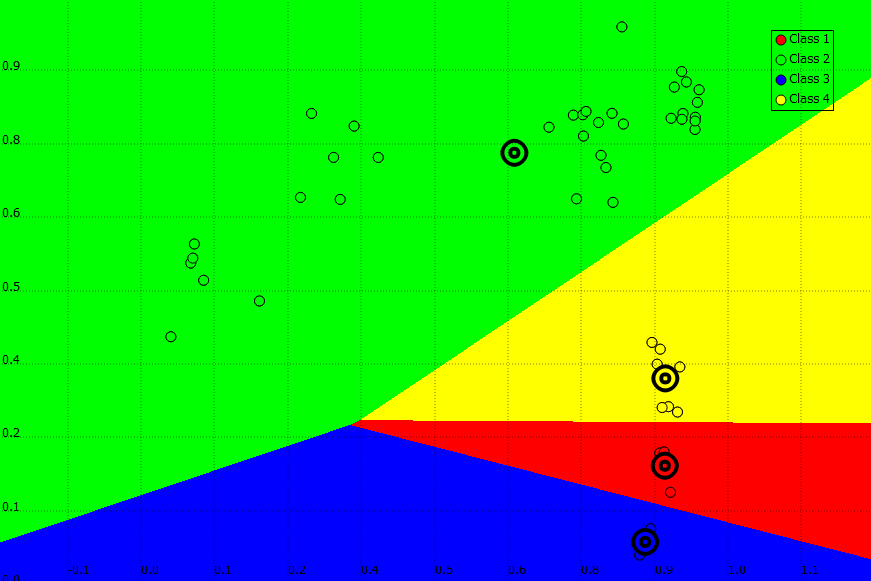
\includegraphics[width=\textwidth]{pictures/dataset_1_Kmeans-4K-L2-wrong}
      \caption{Metric L2}
      \label{fig:dataset_1_Kmeans-4K-L2-bad}
     \end{subfigure}
      ~
    \begin{subfigure}[t]{0.2\textwidth}
      \centering
      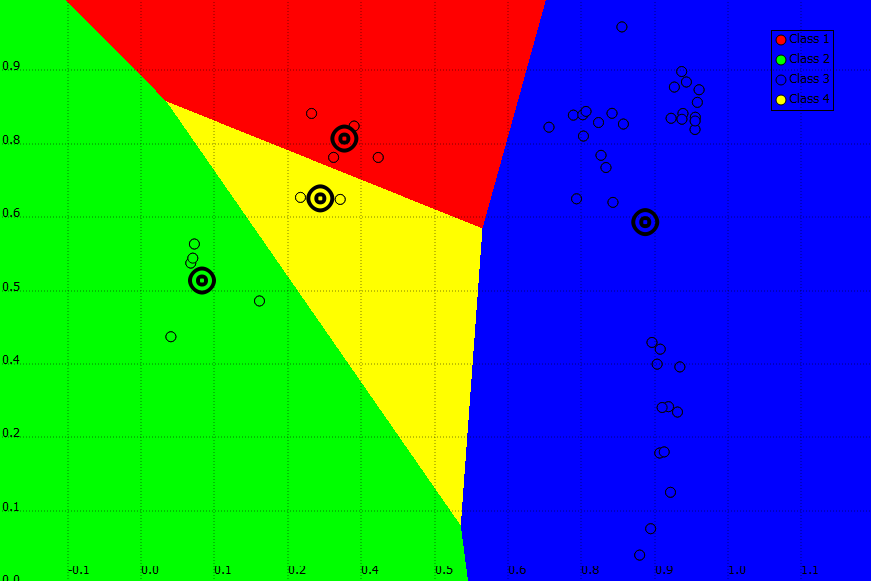
\includegraphics[width=\textwidth]{pictures/dataset_1_Kmeans-4K-L2-wrong2}
      \caption{Metric L2}
      \label{fig:dataset_1_Kmeans-4K-L2-wrong2}
     \end{subfigure}
      ~
    \begin{subfigure}[t]{0.2\textwidth}
      \centering
      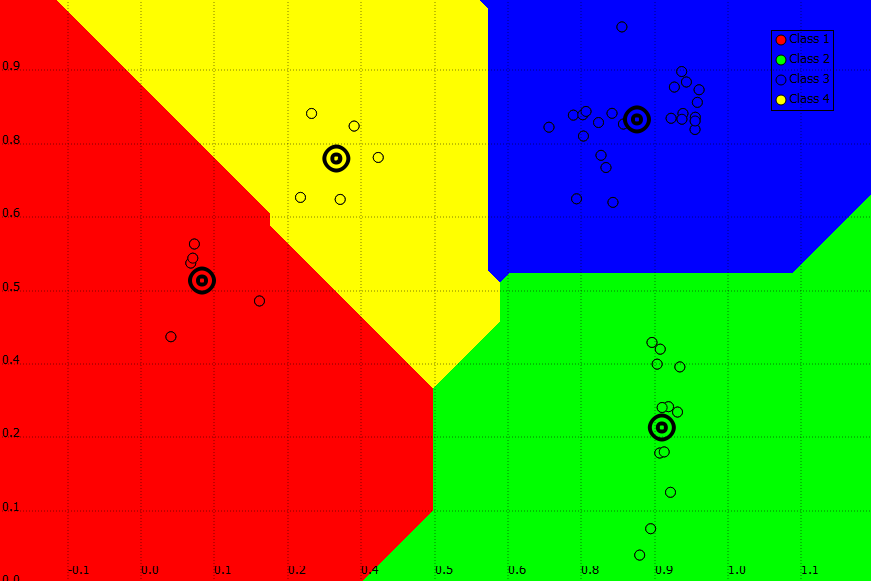
\includegraphics[width=\textwidth]{pictures/dataset_1_Kmeans-4K-Linf-wrong}
      \caption{Metric Linf}
      \label{fig:dataset_1_Kmeans-4K-Linf-wrong}
     \end{subfigure}
      ~
    \begin{subfigure}[t]{0.2\textwidth}
      \centering
      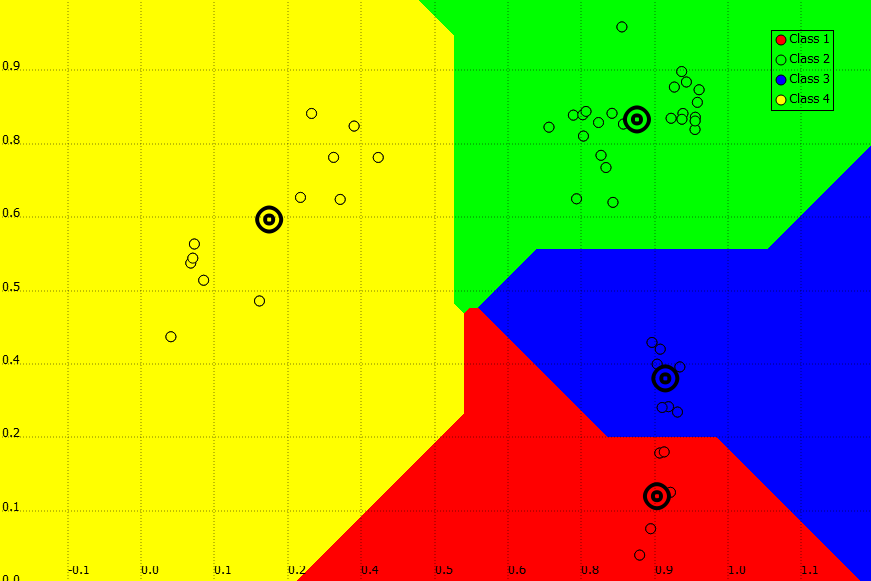
\includegraphics[width=\textwidth]{pictures/dataset_1_Kmeans-4K-Linf-wrong2}
      \caption{Metric Linf}
      \label{fig:dataset_1_Kmeans-4K-Linf-wrong2}
     \end{subfigure}
     \caption{Dataset 1 with incorrect K-Means clustering, metrics L2 and Linf and K=4}
     \label{fig:bad_kmeans}
\end{figure}
%End bad results

Finally, K-Means behaviour was tested for different values of K (see Figure \ref{fig:kmeans_differentK}). Since clustering does not use the label of each point, the separation of datapoints is done according to the position of the points in the PCA projection. For dataset 1, the classes Chairs and Pens are quite close in the PCA projection (see Figure \ref{fig:dataset_1_labelized}). As such, when the cluster number is smaller than the total number of classes as in Figure \ref{fig:dataset_1_Kmeans-L2-3K}, the classes Chairs and Pens are left in the same cluster.

%Different values of K
\begin{figure}[H]
\centering
    \begin{subfigure}[t]{0.2\textwidth}
      \centering
      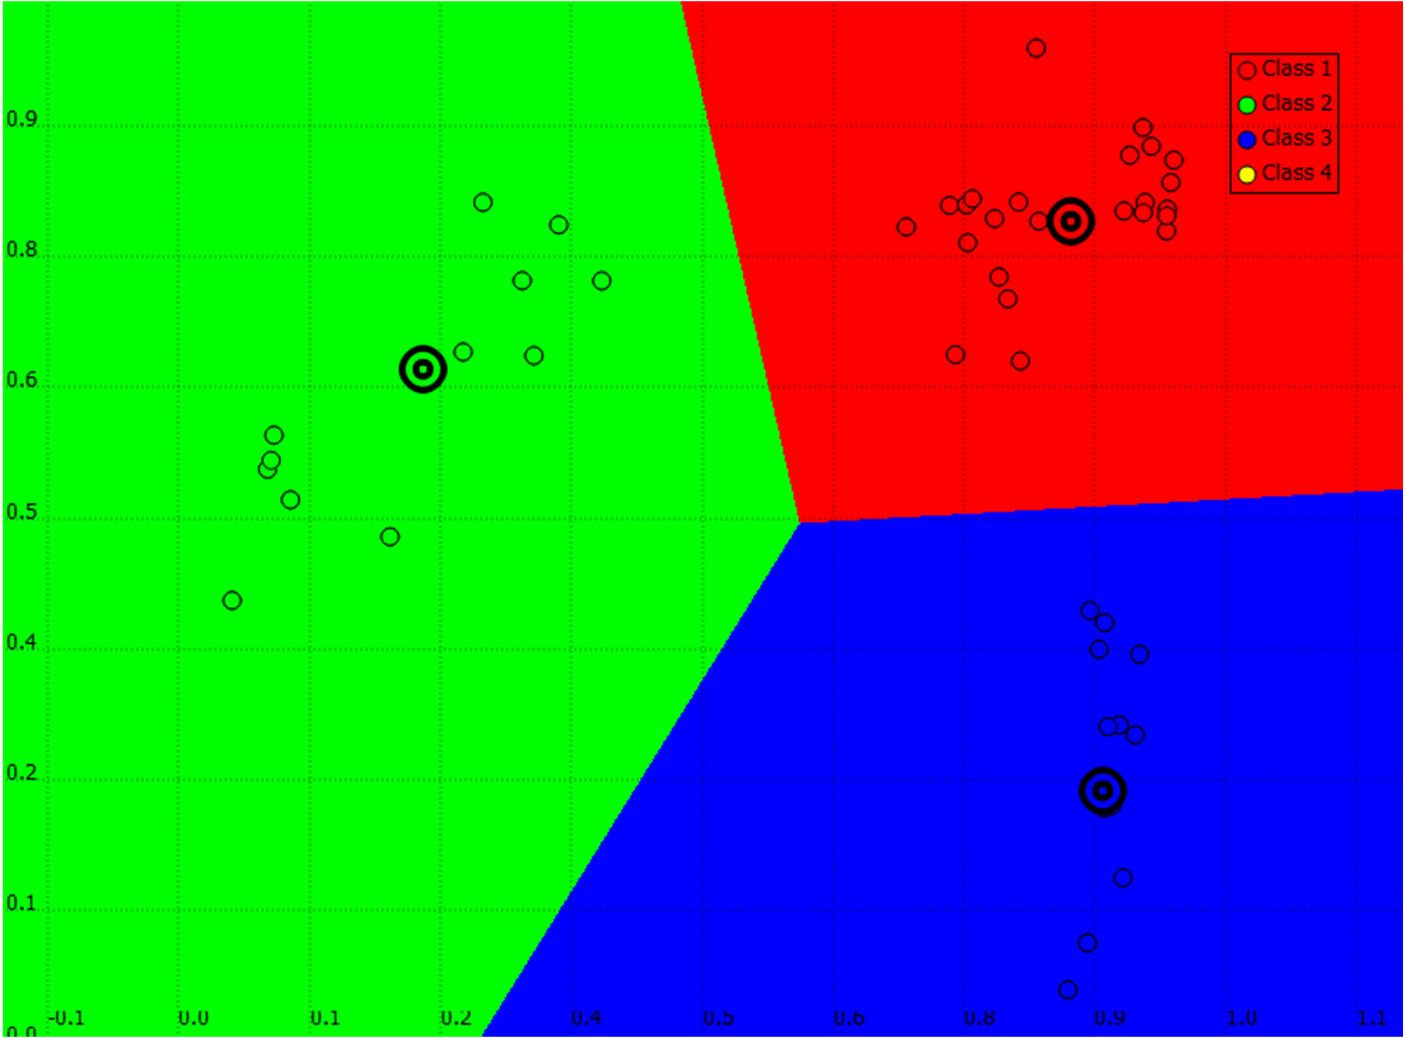
\includegraphics[width=\textwidth]{pictures/dataset_1_Kmeans-L2-3K}
      \caption{K = 3}
      \label{fig:dataset_1_Kmeans-L2-3K}
     \end{subfigure}
      ~
    \begin{subfigure}[t]{0.2\textwidth}
      \centering
      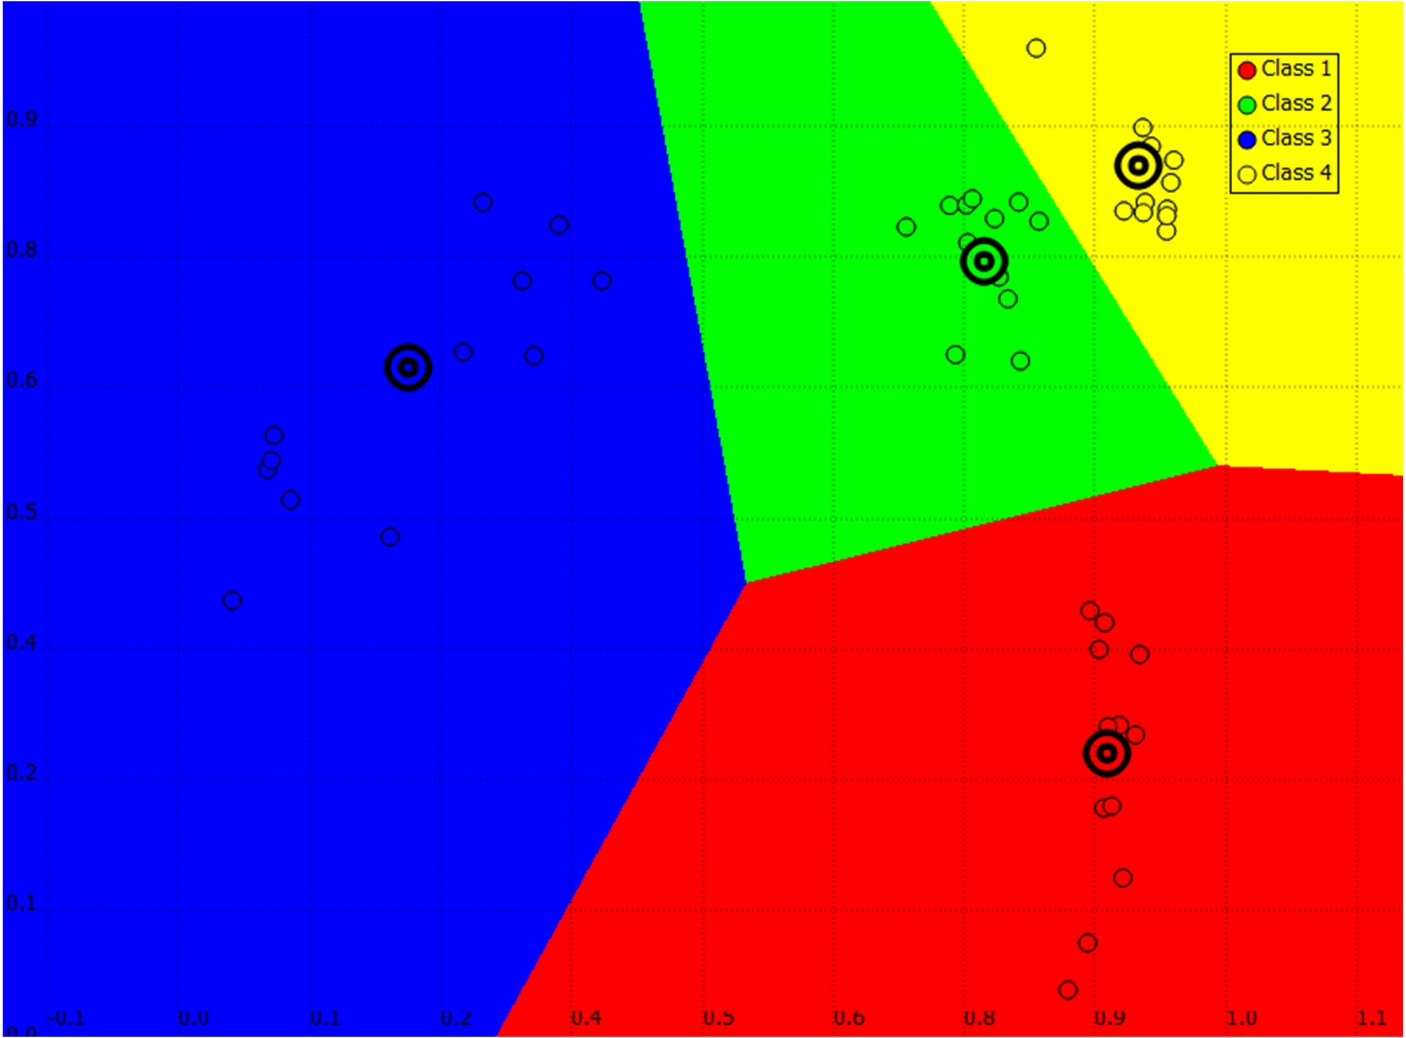
\includegraphics[width=\textwidth]{pictures/dataset_1_Kmeans-L2-4K}
      \caption{K = 4}
      \label{fig:dataset_1_Kmeans-L2-4K}
     \end{subfigure}
      ~
    \begin{subfigure}[t]{0.2\textwidth}
      \centering
      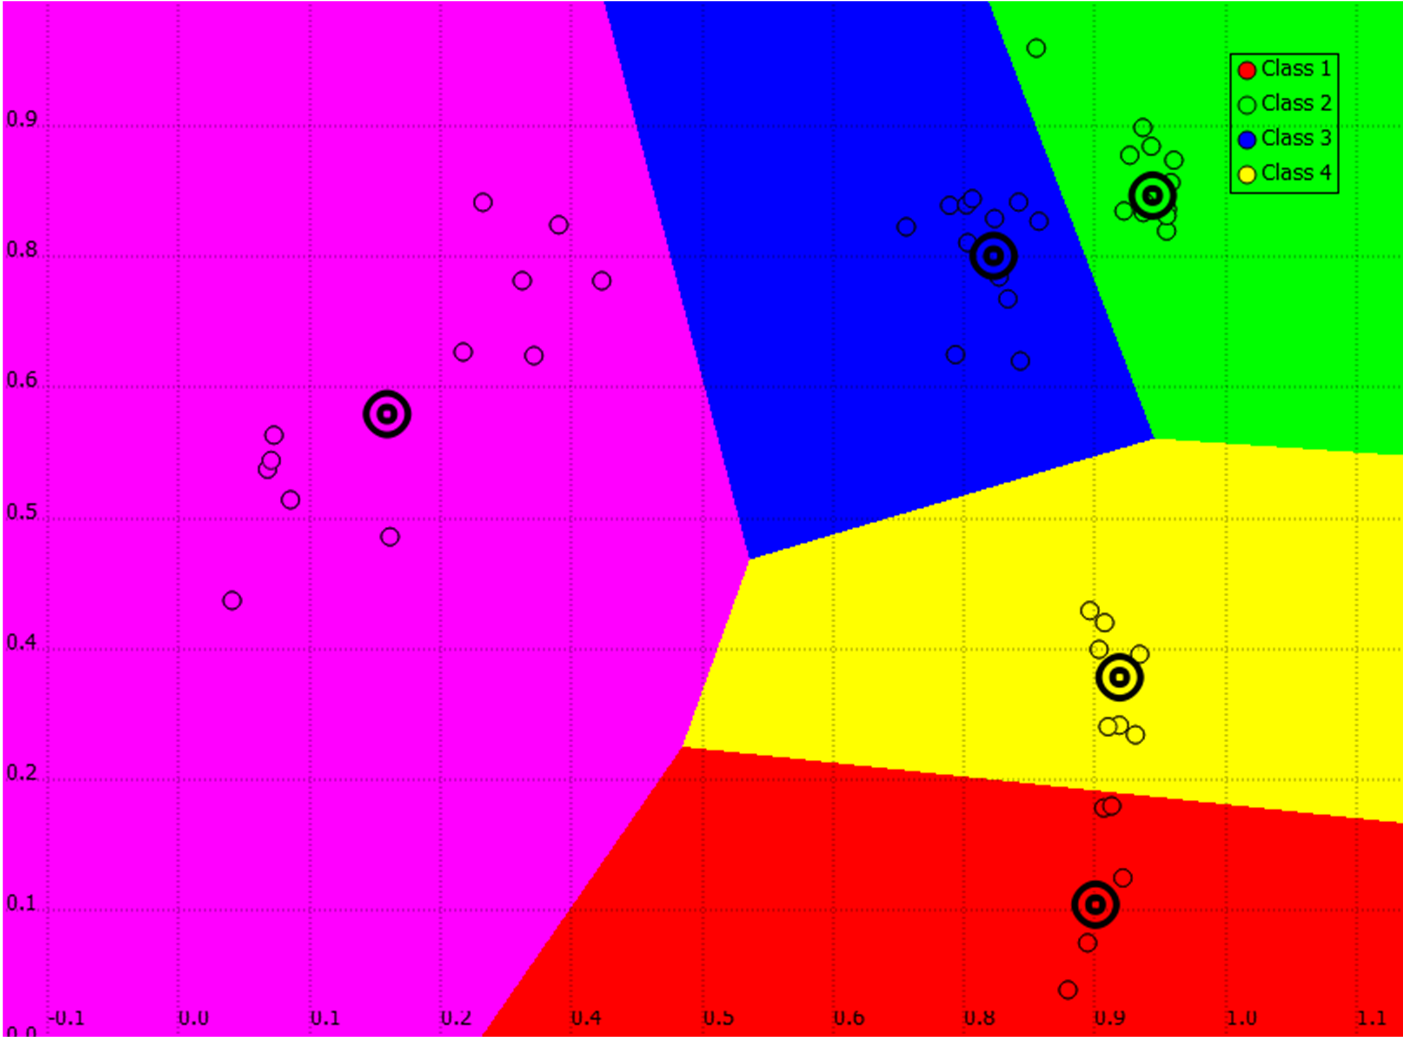
\includegraphics[width=\textwidth]{pictures/dataset_1_Kmeans-L2-5K}
      \caption{K = 5}
      \label{fig:dataset_1_Kmeans-L2-5K}
     \end{subfigure}
      ~
    \begin{subfigure}[t]{0.2\textwidth}
      \centering
      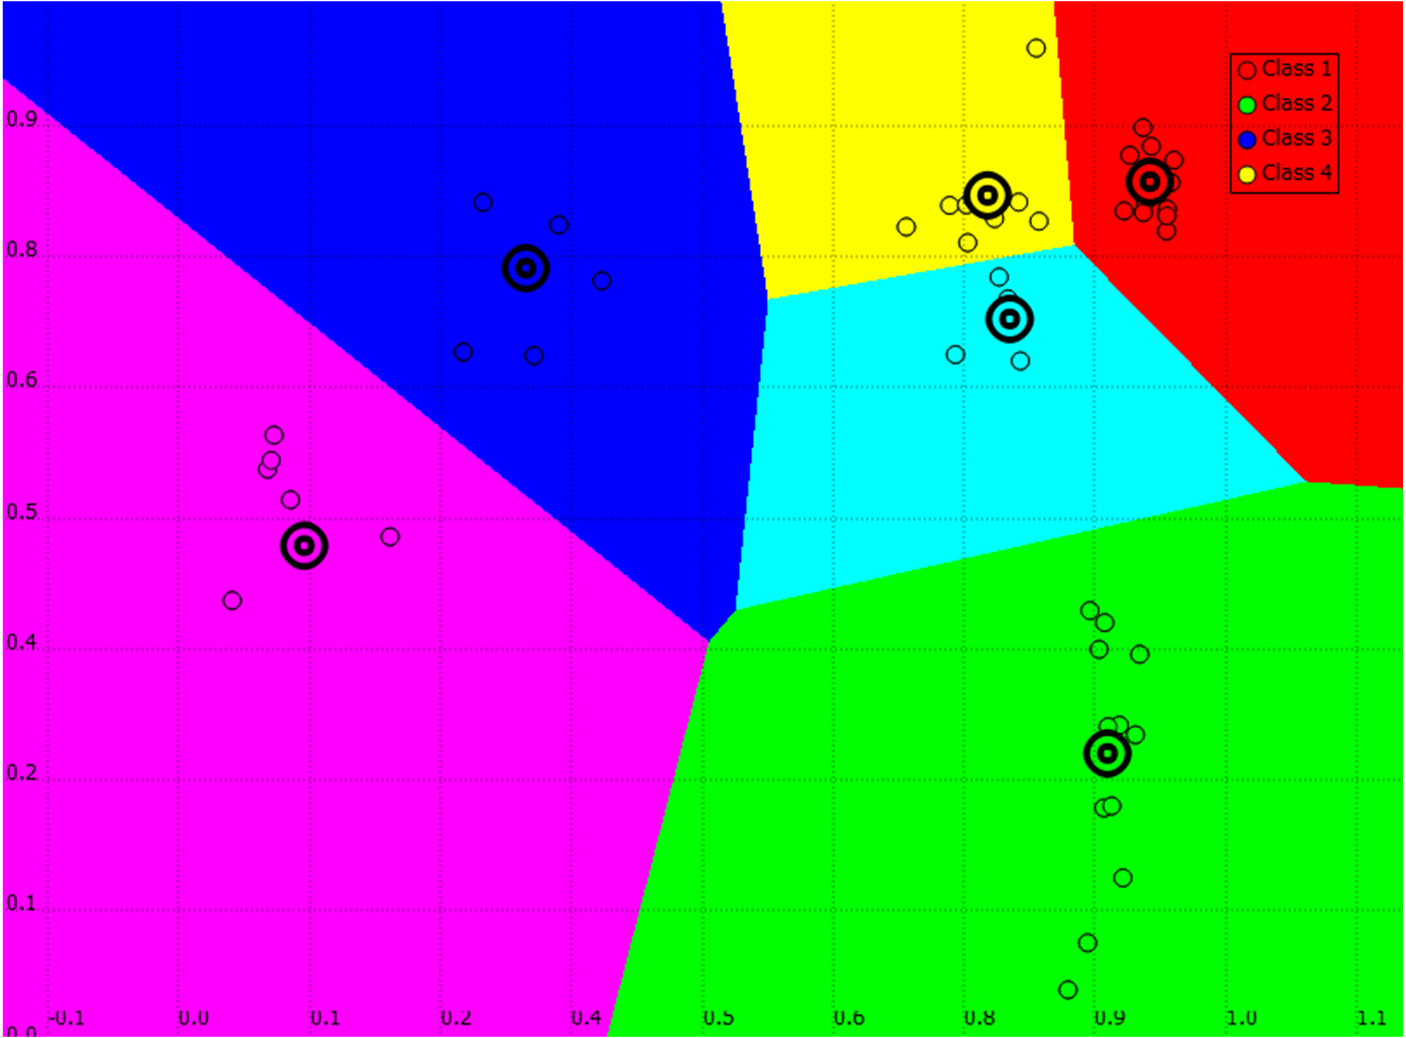
\includegraphics[width=\textwidth]{pictures/dataset_1_Kmeans-L2-6K}
      \caption{K = 6}
      \label{fig:dataset_1_Kmeans-L2-6K}
     \end{subfigure}
     \caption{Dataset 1 with K-Means clustering, Euclidean metrics and different value of K}
     \label{fig:kmeans_differentK}
\end{figure}



\subsection{Soft K-Means}

The hyperparameters for the soft K-means method are:
\begin{itemize}
\item the number of clusters;
\item the stiffness $\beta$.
\end{itemize}

In Figure \ref{fig:soft_kmeans_varyb}, results for K=4 and different values of $\beta$ are shown. The higher the value of $\beta$, the more similar soft K-Means becomes to hard K-Means. When the stiffness is too low, the classes are difficult to distinguish. From $\beta = 30$, the 4 classes are clearly distinguished and correctly clustered.  

%Different betas
\begin{figure}[H]
\centering
    \begin{subfigure}[t]{0.2\textwidth}
      \centering
      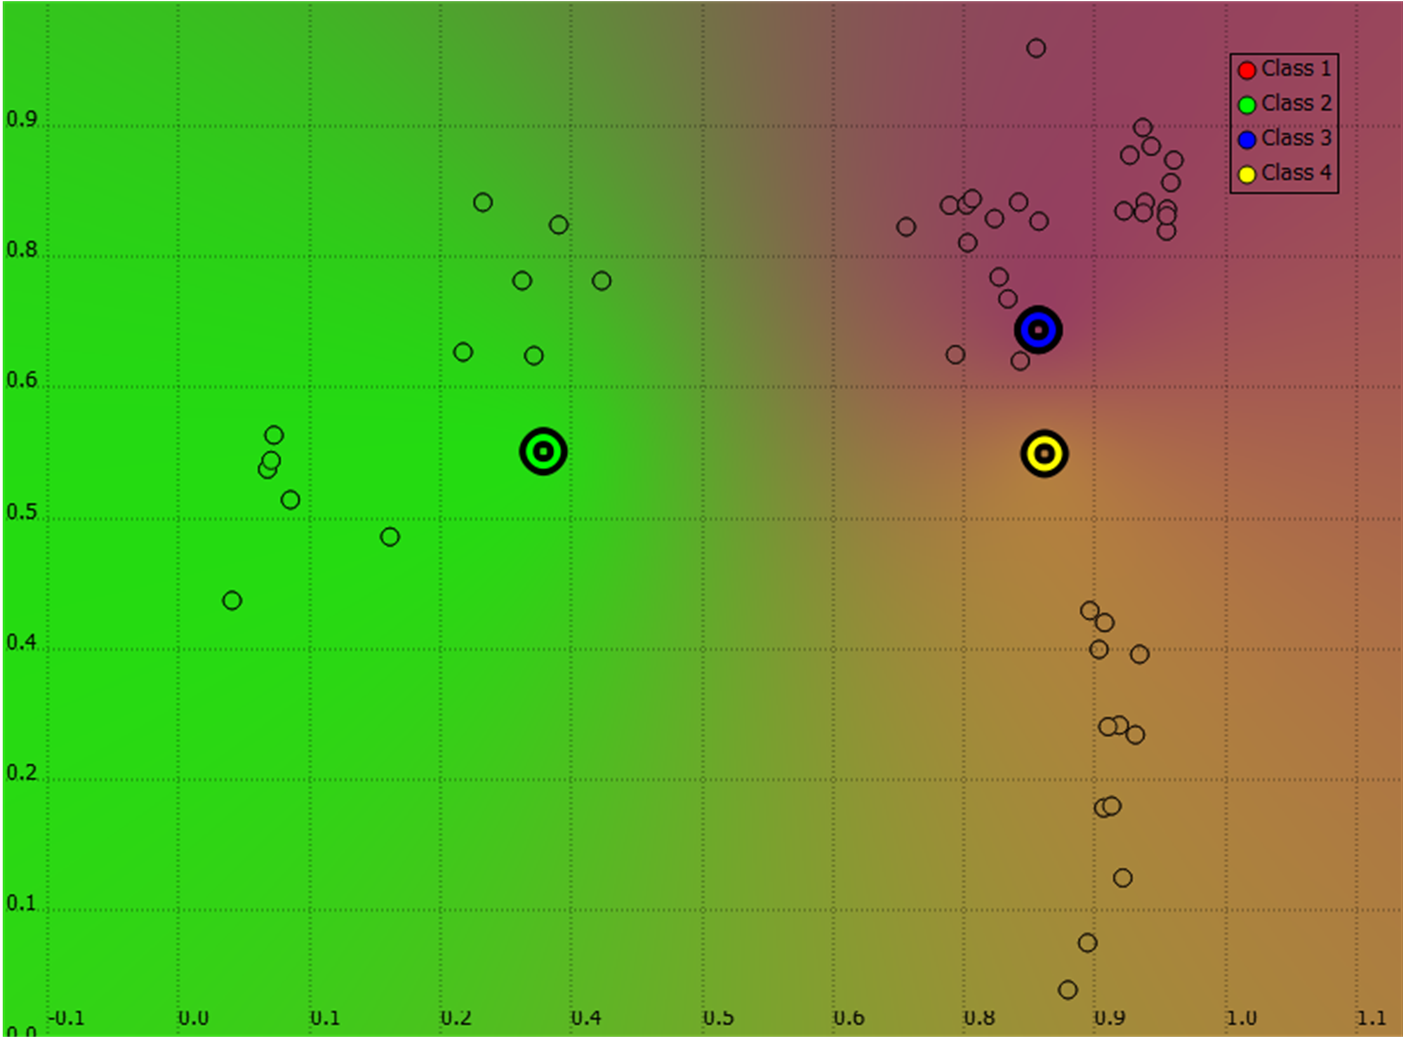
\includegraphics[width=\textwidth]{pictures/dataset_1_soft-Kmeans-4K-beta5}
      \caption{$\beta = 5$}
      \label{fig:dataset_1_soft-Kmeans-4K-beta5}
     \end{subfigure}
      ~
    \begin{subfigure}[t]{0.2\textwidth}
      \centering
      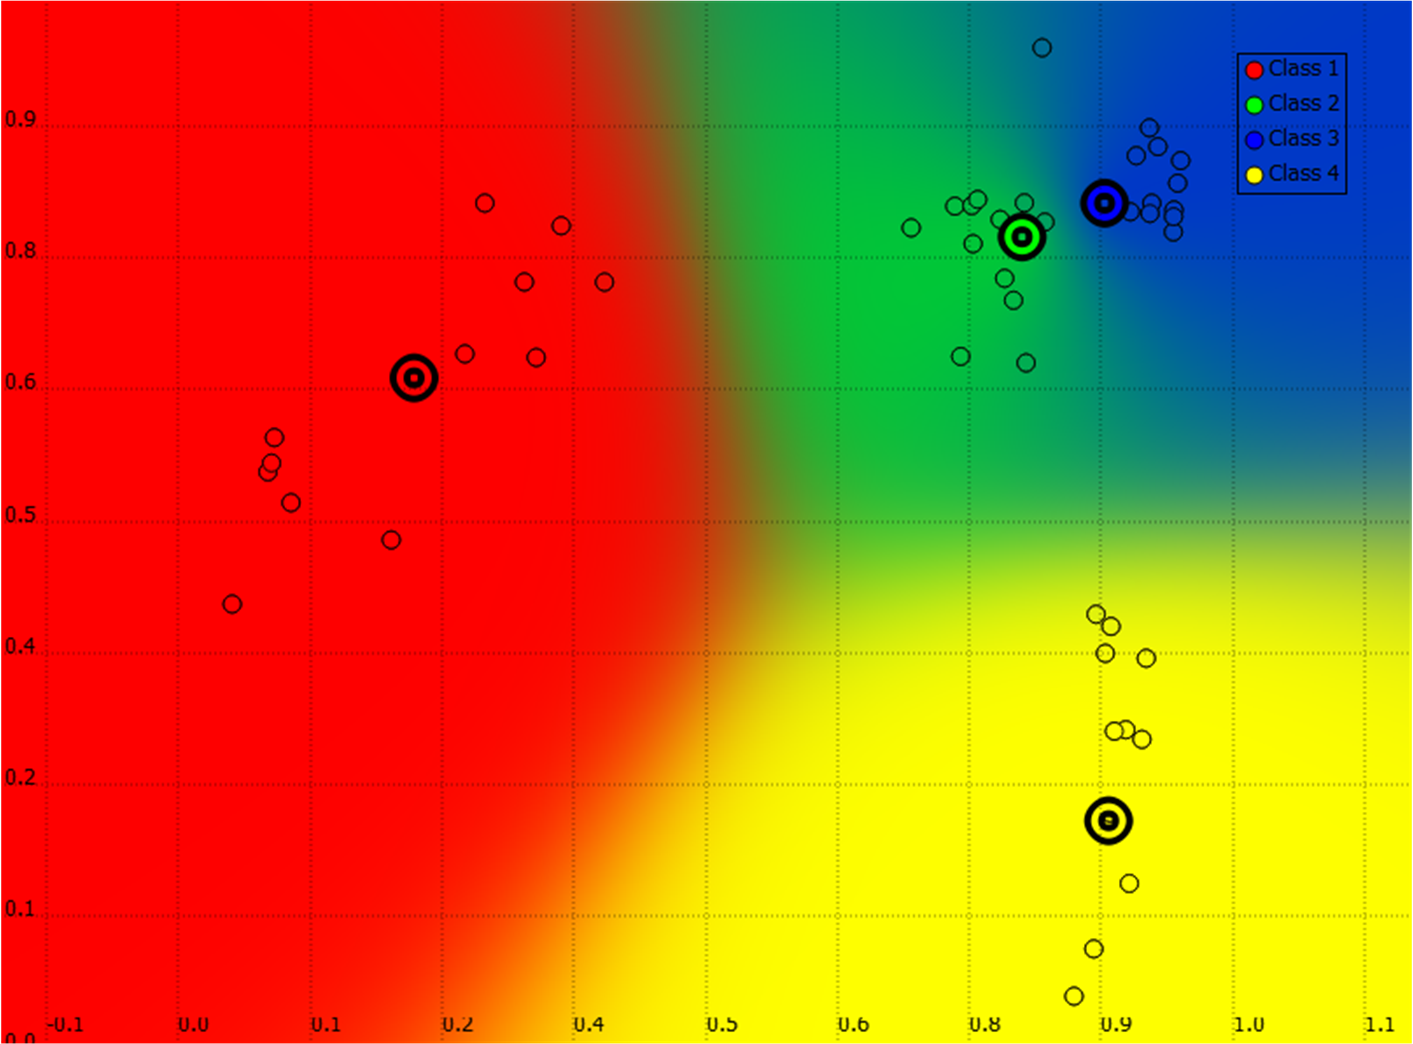
\includegraphics[width=\textwidth]{pictures/dataset_1_soft-Kmeans-4K-beta15}
      \caption{$\beta = 15$}
      \label{fig:dataset_1_soft-Kmeans-4K-beta15}
     \end{subfigure}
      ~
    \begin{subfigure}[t]{0.2\textwidth}
      \centering
      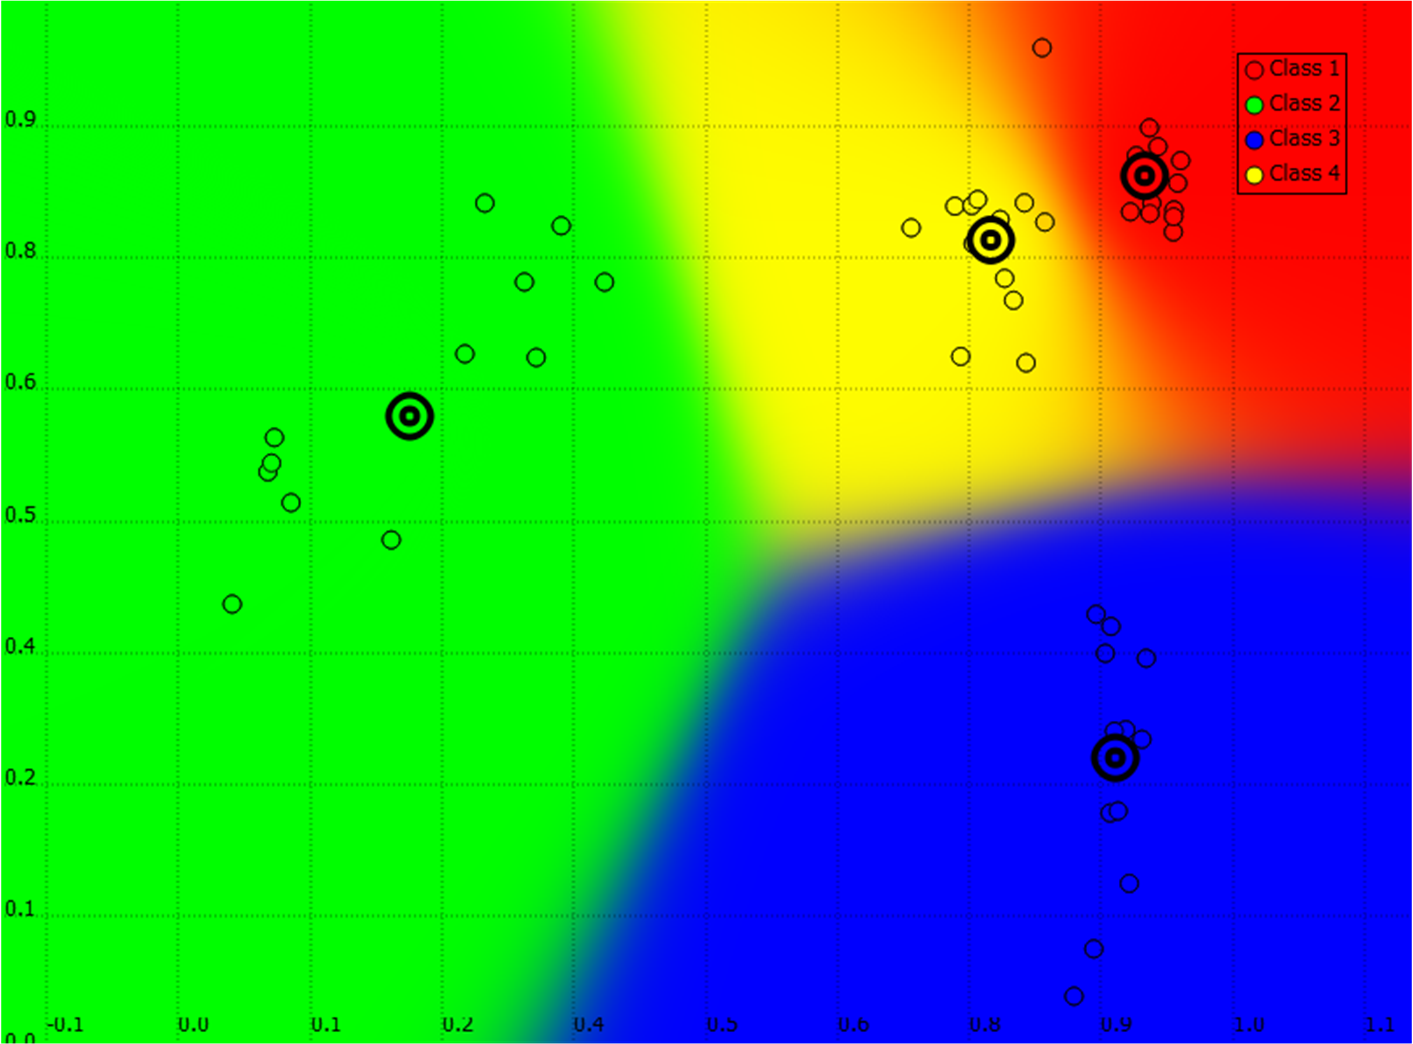
\includegraphics[width=\textwidth]{pictures/dataset_1_soft-Kmeans-4K-beta30}
      \caption{$\beta = 30$}
      \label{fig:dataset_1_soft-Kmeans-4K-beta30}
     \end{subfigure}
      ~
    \begin{subfigure}[t]{0.2\textwidth}
      \centering
      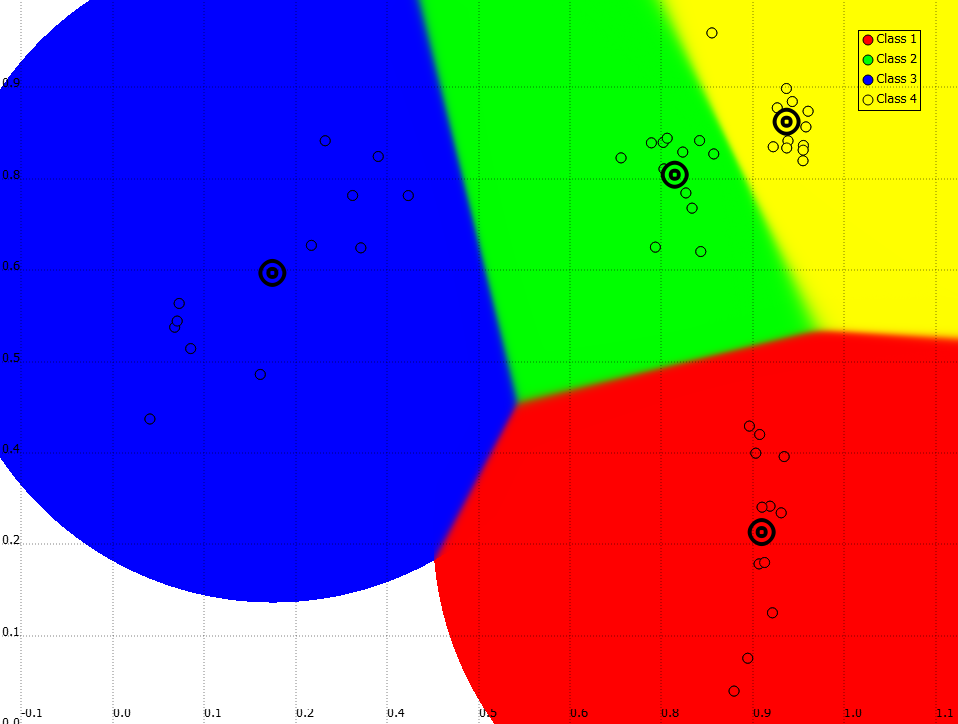
\includegraphics[width=\textwidth]{pictures/dataset_1_soft-Kmeans-4K-beta200}
      \caption{$\beta = 200$}
      \label{fig:dataset_1_soft-Kmeans-4K-beta200}
     \end{subfigure}
     \caption{Dataset 1 with soft K-Means clustering, K = 4 and different value of $\beta$}
     \label{fig:soft_kmeans_varyb}
\end{figure}
%End different betas

It can be noticed that the results for soft K-Means when varying the K don't differ considerably from what obtained with hard K-Means, as shown in Figure \ref{fig:soft_kmeans_varyk}.

%different Ks
\begin{figure}[H]
\centering
    \begin{subfigure}[t]{0.2\textwidth}
      \centering
      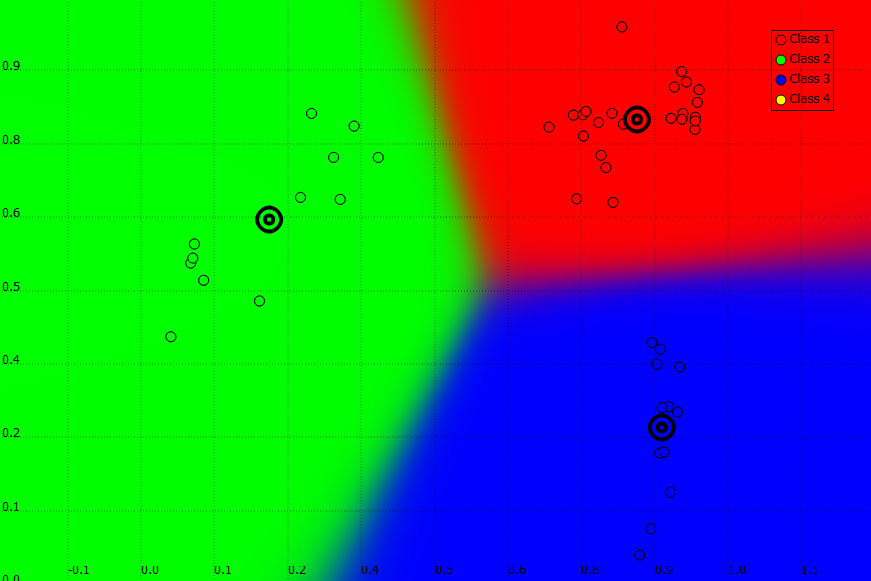
\includegraphics[width=\textwidth]{pictures/dataset_1_soft-Kmeans-3K-beta30}
      \caption{K=3}
      \label{fig:dataset_1_soft-Kmeans-3K-beta30}
     \end{subfigure}
      ~
    \begin{subfigure}[t]{0.2\textwidth}
      \centering
      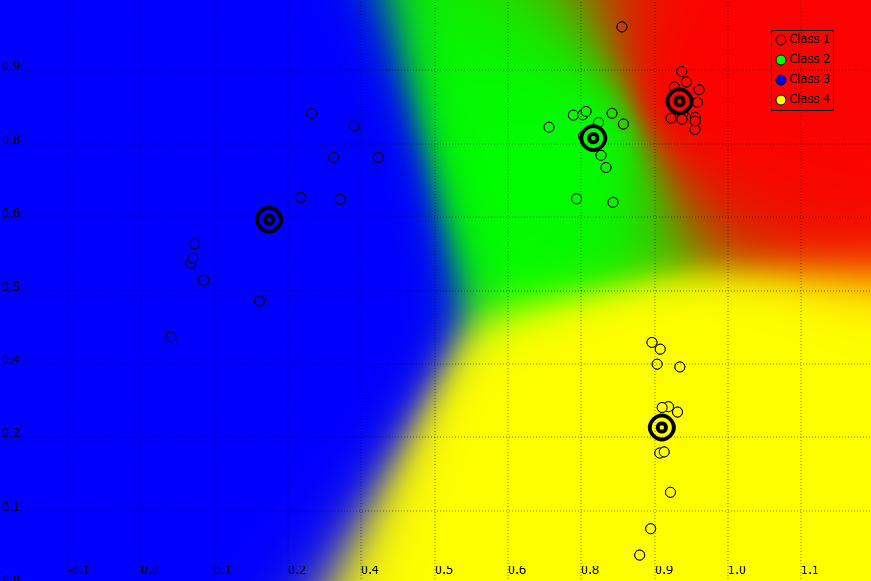
\includegraphics[width=\textwidth]{pictures/dataset_1_soft-Kmeans-4K-beta30-2}
      \caption{K=4}
      \label{fig:dataset_1_soft-Kmeans-4K-beta30-2}
     \end{subfigure}
      ~
    \begin{subfigure}[t]{0.2\textwidth}
      \centering
      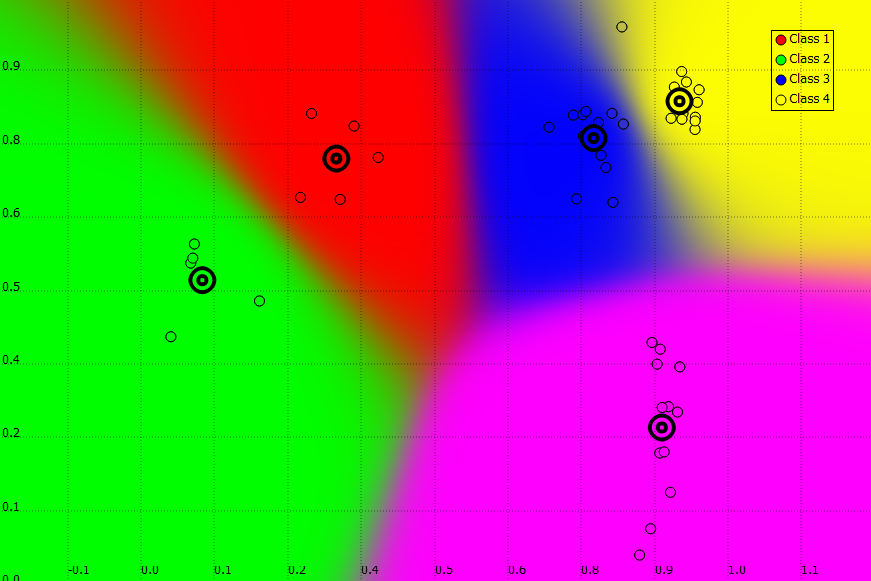
\includegraphics[width=\textwidth]{pictures/dataset_1_soft-Kmeans-5K-beta30}
      \caption{K=5}
      \label{fig:dataset_1_soft-Kmeans-5K-beta30}
     \end{subfigure}
      ~
    \begin{subfigure}[t]{0.2\textwidth}
      \centering
      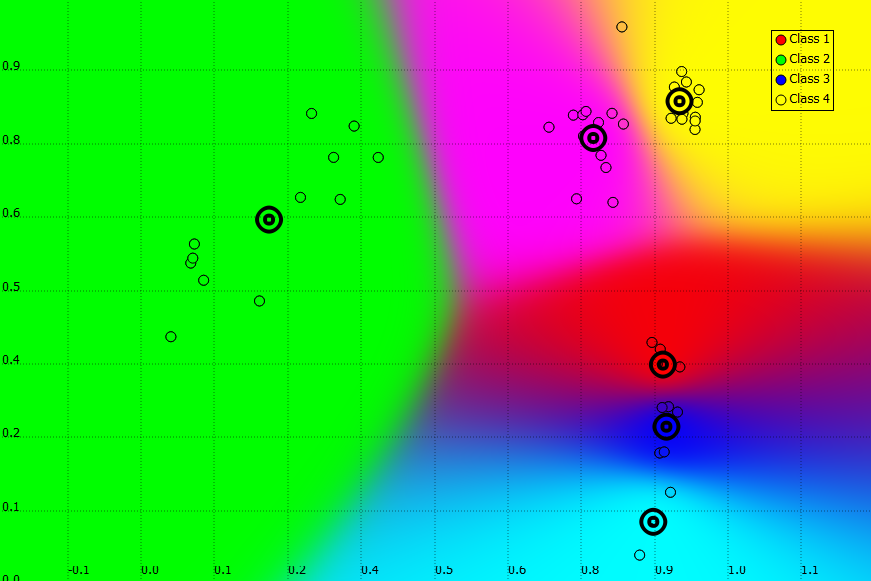
\includegraphics[width=\textwidth]{pictures/dataset_1_soft-Kmeans-6K-beta30}
      \caption{K=6}
      \label{fig:dataset_1_soft-Kmeans-6K-beta30}
     \end{subfigure}
     \caption{Dataset 1 with soft K-Means clustering,$\beta = 30$ and different values of K}
     \label{fig:soft_kmeans_varyk}
\end{figure}
%End different Ks

\subsubsection*{Initialization}

The methods above apply a random initialisation of the cluster centers. The effect of this random procedure can be observed in Figure \ref{fig:kmeans_init}. In particular, Figures \ref{fig:K-Means-4K-beta-30-it1} to \ref{fig:K-Means-4K-beta-30-it10} show an initialization that results in an incorrect clustering, while Figures \ref{fig:K-Means-4K-beta-30-it1-2} to \ref{fig:K-Means-4K-beta-30-it6-2} show a correct clustering starting from iteration 3.

%Different iterations for kmeans
\begin{figure}[H]
\centering
    \begin{subfigure}[t]{0.2\textwidth}
      \centering
      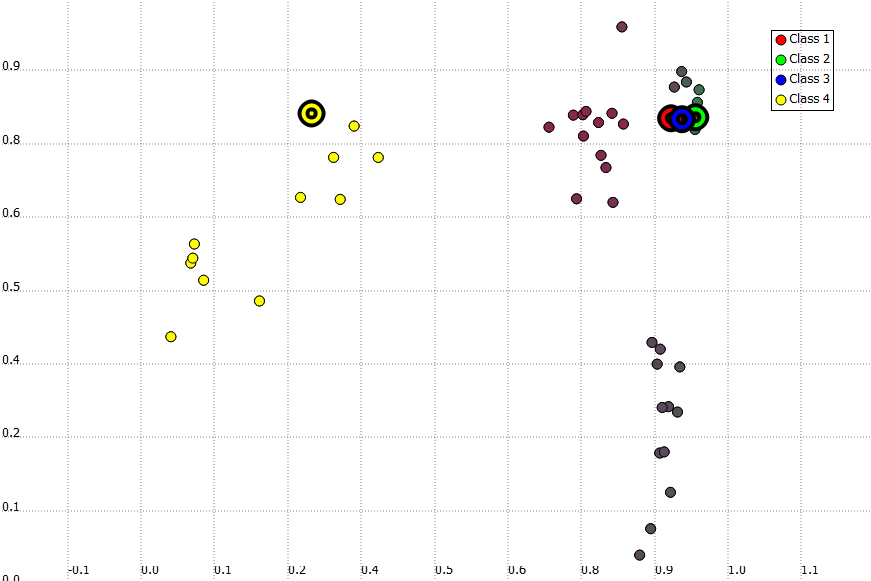
\includegraphics[width=\textwidth]{pictures/K-Means-4K-beta-30-it1.png}
      \caption{Iteration 1}
      \label{fig:K-Means-4K-beta-30-it1}
     \end{subfigure}
      ~
    \begin{subfigure}[t]{0.2\textwidth}
      \centering
      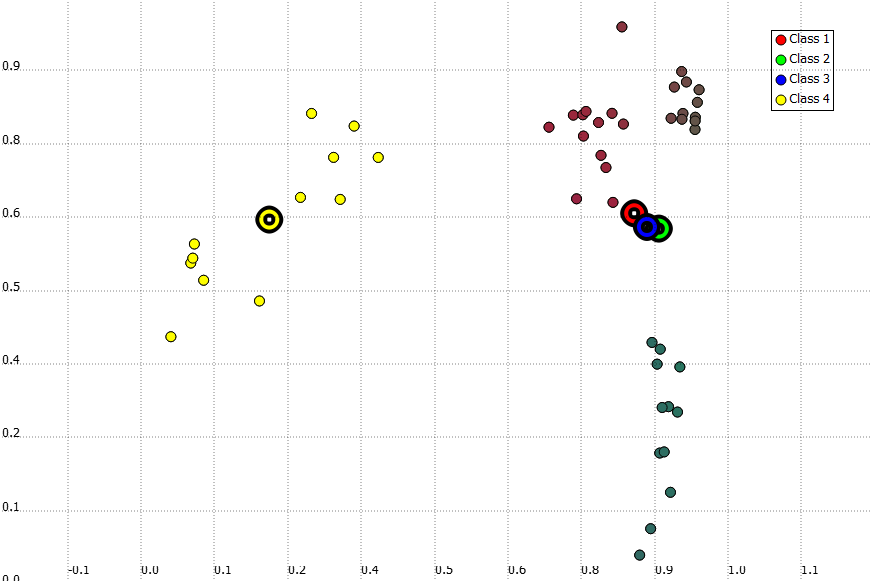
\includegraphics[width=\textwidth]{pictures/K-Means-4K-beta-30-it2.png}
      \caption{Iteration 2}
      \label{fig:K-Means-4K-beta-30-it2}
     \end{subfigure}
      ~
    \begin{subfigure}[t]{0.2\textwidth}
      \centering
      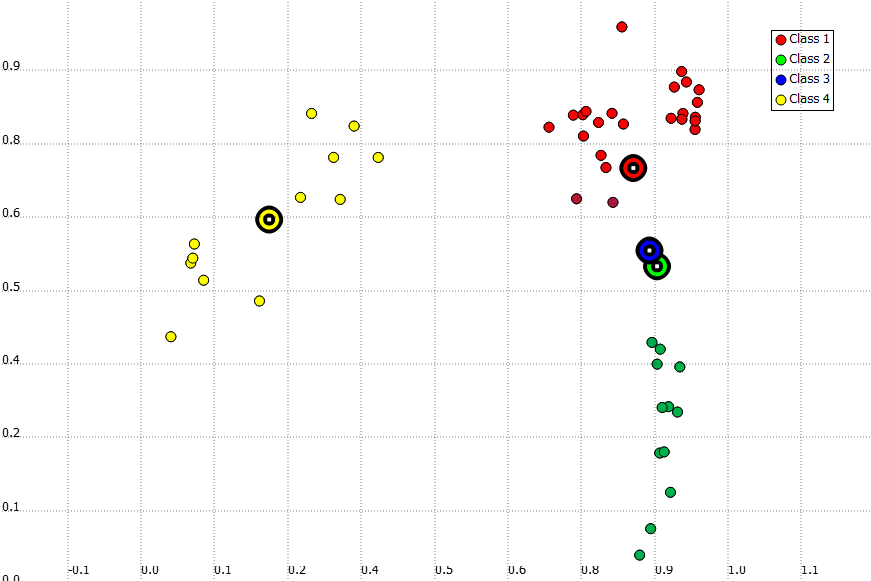
\includegraphics[width=\textwidth]{pictures/K-Means-4K-beta-30-it3.png}
      \caption{Iteration 3}
      \label{fig:K-Means-4K-beta-30-it3}
     \end{subfigure}
      ~
    \begin{subfigure}[t]{0.2\textwidth}
      \centering
      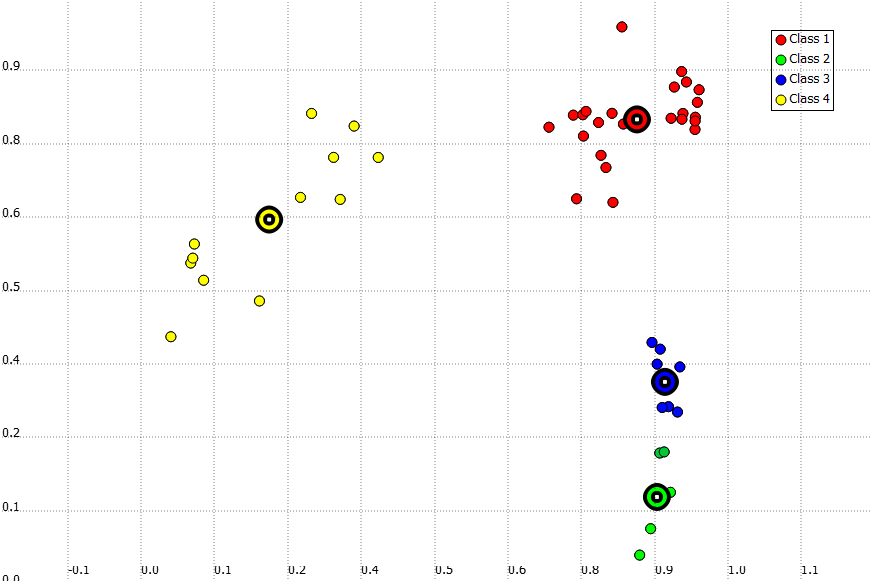
\includegraphics[width=\textwidth]{pictures/K-Means-4K-beta-30-it10.png}
      \caption{Iteration 10}
      \label{fig:K-Means-4K-beta-30-it10}
     \end{subfigure}
     ~
     \begin{subfigure}[t]{0.2\textwidth}
      \centering
      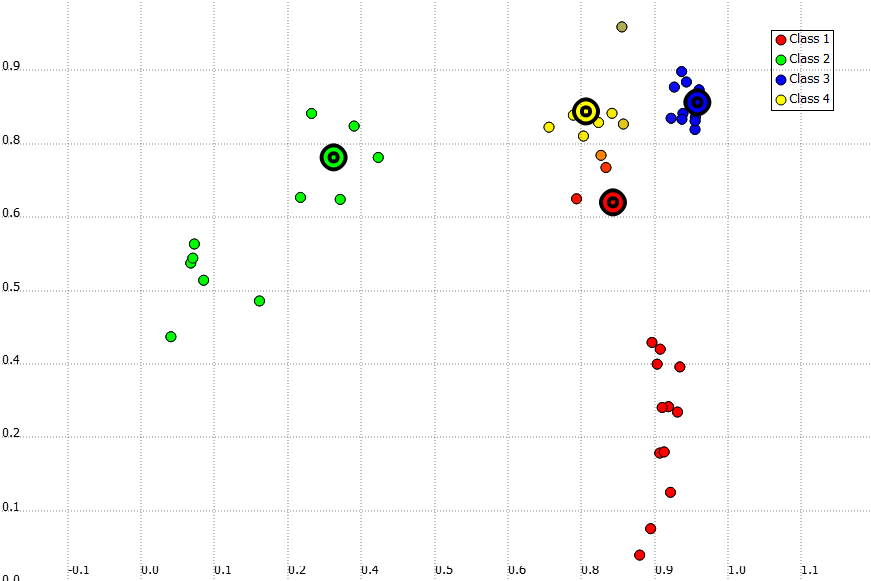
\includegraphics[width=\textwidth]{pictures/K-Means-4K-beta-30-it1(2).png}
      \caption{Iteration 1}
      \label{fig:K-Means-4K-beta-30-it1-2}
     \end{subfigure}
      ~
    \begin{subfigure}[t]{0.2\textwidth}
      \centering
      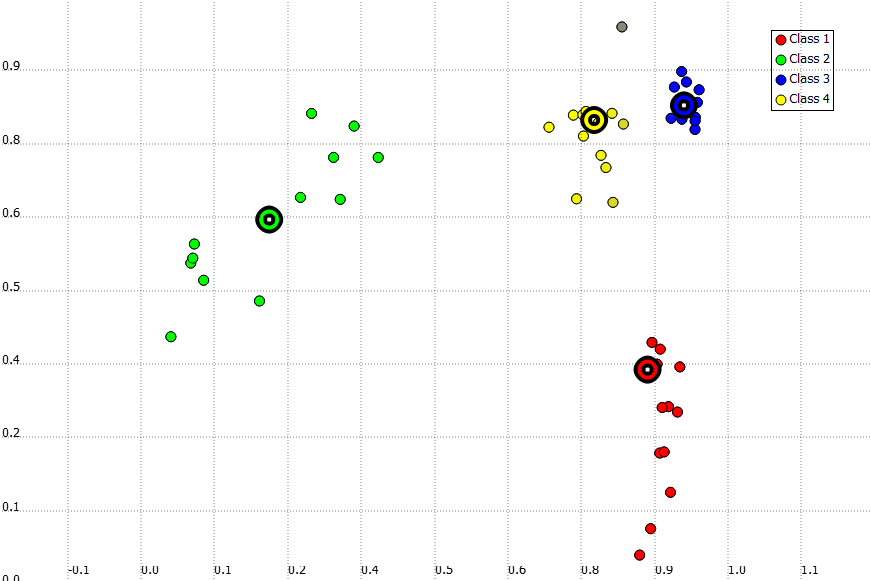
\includegraphics[width=\textwidth]{pictures/K-Means-4K-beta-30-it2(2).png}
      \caption{Iteration 2}
      \label{fig:K-Means-4K-beta-30-it2-2}
     \end{subfigure}
      ~
    \begin{subfigure}[t]{0.2\textwidth}
      \centering
      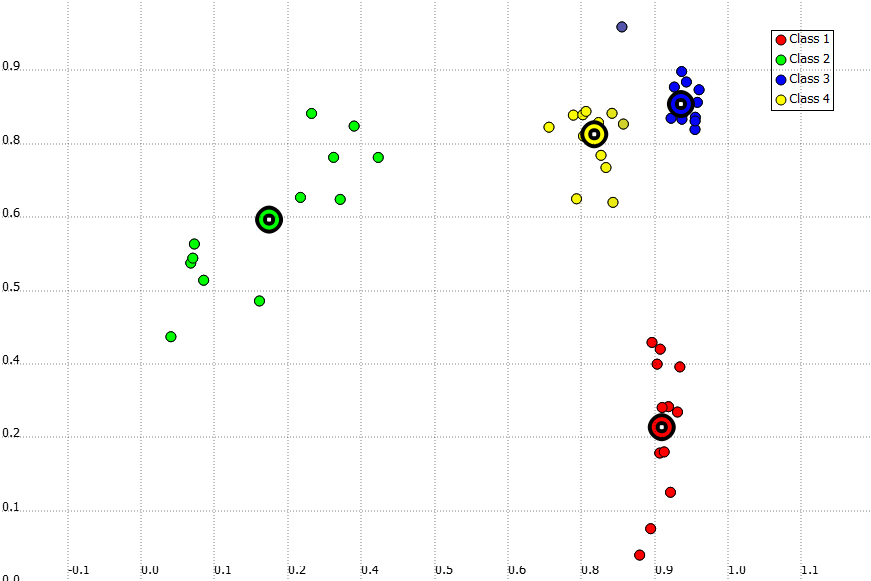
\includegraphics[width=\textwidth]{pictures/K-Means-4K-beta-30-it3(2).png}
      \caption{Iteration 3}
      \label{fig:K-Means-4K-beta-30-it3-2}
     \end{subfigure}
      ~
    \begin{subfigure}[t]{0.2\textwidth}
      \centering
      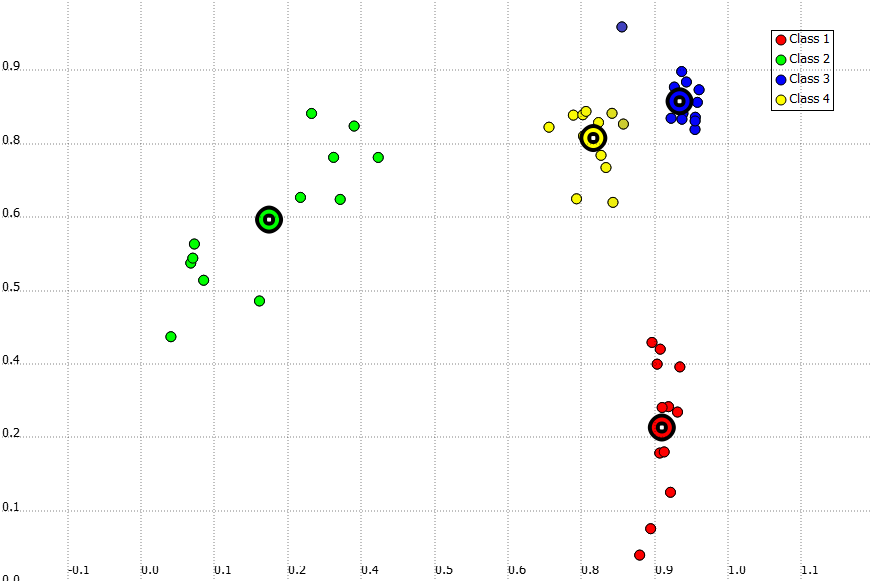
\includegraphics[width=\textwidth]{pictures/K-Means-4K-beta-30-it6(2).png}
      \caption{Iteration 6}
      \label{fig:K-Means-4K-beta-30-it6-2}
     \end{subfigure}
     \caption{Dataset 1 with soft K-Means clustering for K=4 and $\beta=30$, showing effects of random initialization}
     \label{fig:kmeans_init}
\end{figure}


\subsection{DBSCAN}

The hyperparameters for the DBScan method are:
\begin{itemize}
\item the minimum number of points in a cluster MinPts;
\item the size of neighborhood $\epsilon$.
\end{itemize}

It can be noticed that when the number of Minpoints increases (see Figure \ref{fig:DBScan_varyminpt}), the smaller clusters are lost, and more and more points are considered outliers as the $\epsilon$ doesn't change.

%DBScan varying MinPts
\begin{figure}[H]
\centering
    \begin{subfigure}[t]{0.2\textwidth}
      \centering
      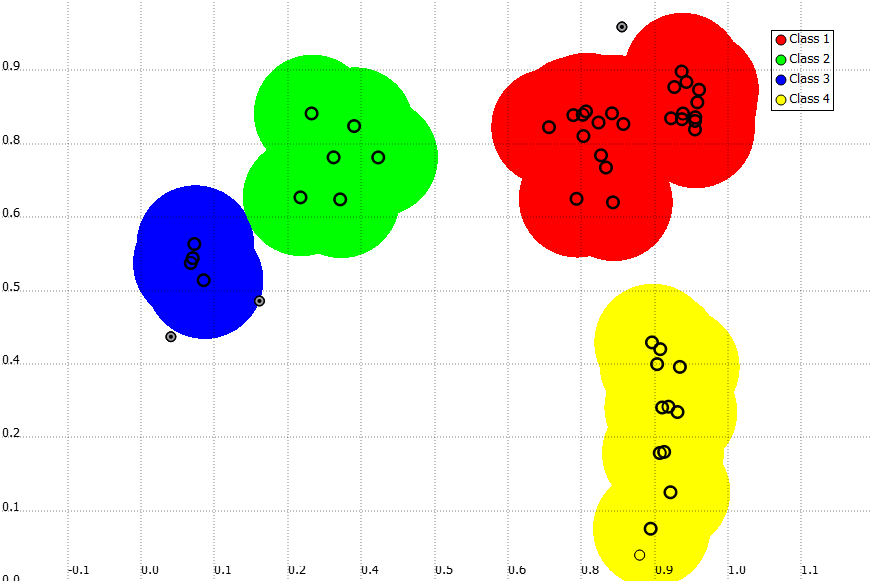
\includegraphics[width=\textwidth]{pictures/DBSCAN-epsilon01-Minpoint-2}
      \caption{$Minpoints = 2$}
      \label{fig:DBSCAN-epsilon01-Minpoint-2}
     \end{subfigure}
      ~
    \begin{subfigure}[t]{0.2\textwidth}
      \centering
      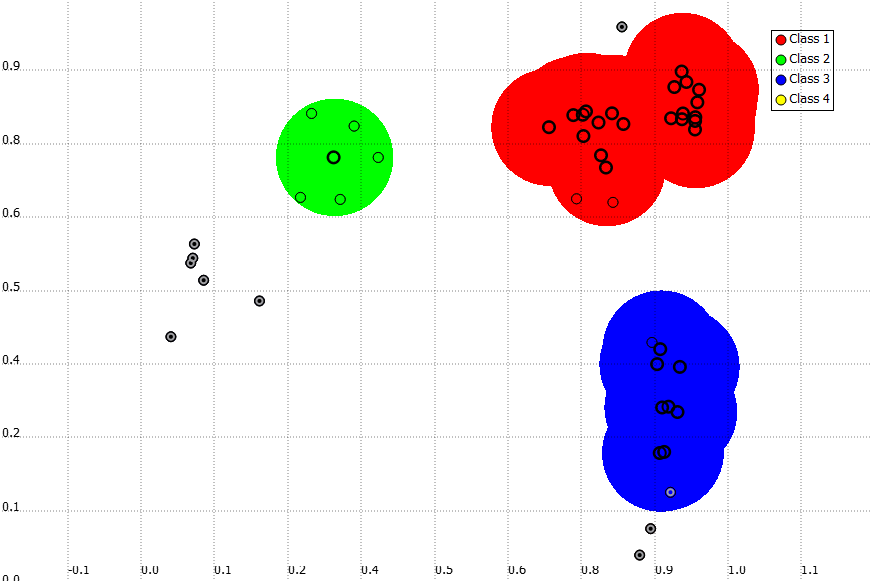
\includegraphics[width=\textwidth]{pictures/DBSCAN-epsilon01-Minpoint-4}
      \caption{$Minpoints = 4$}
      \label{fig:DBSCAN-epsilon01-Minpoint-4}
     \end{subfigure}
      ~
    \begin{subfigure}[t]{0.2\textwidth}
      \centering
      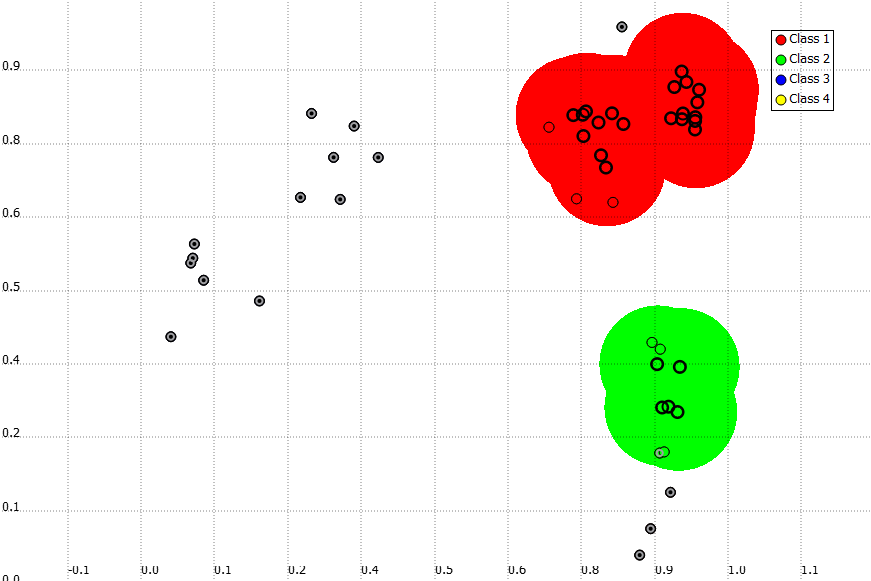
\includegraphics[width=\textwidth]{pictures/DBSCAN-epsilon01-Minpoint-6}
      \caption{$Minpoints = 6$}
      \label{fig:DBSCAN-epsilon01-Minpoint-6}
     \end{subfigure}
      ~
    \begin{subfigure}[t]{0.2\textwidth}
      \centering
      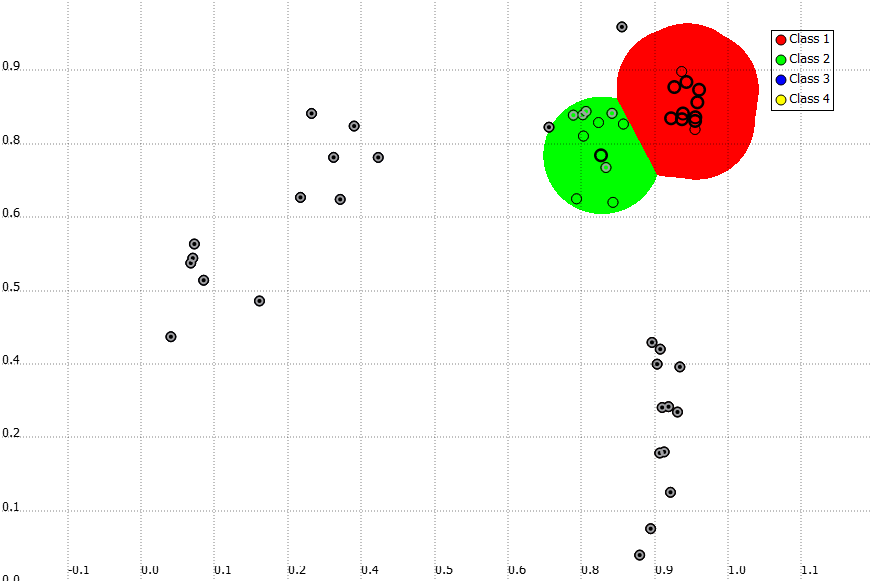
\includegraphics[width=\textwidth]{pictures/DBSCAN-epsilon01-Minpoint-10}
      \caption{$Minpoints = 10$}
      \label{fig:DBSCAN-epsilon01-Minpoint-10}
     \end{subfigure}
     \caption{Dataset 1 with DBSCAN clustering, $\epsilon = 0.1 $ and different value of $Minpoints$}
     \label{fig:DBScan_varyminpt}
\end{figure}
%DBScan varying MinPts

The value of $\epsilon$ was then varied for a fixed Minpt = 2, as it can be seen in Figure \ref{fig:DBScan_varyeps}.
For smaller values of $\epsilon$ (as Figure \ref{fig:DBSCAN-Minpoint-2-epsilon005}), the size of the clusters is expectedly smaller, and as the density of the dataset is not uniform, many outliers are present. This method results in  clusters than are not necessarily globular, which is an advantage compared to K-Means for this particular dataset, but it clusters datapoints whose inter-distance is smaller than $\epsilon$. As such, in this particular case, the classes Chairs and Pens can be distinguished only for small values of $\epsilon$, which do not cluster well the other classes as their density is lower. When the value of $\epsilon$ is higher, (i.e. Figure \ref{fig:DBSCAN-Minpoint-2-epsilon02}), the classes Bananas and Watches are correctly clustered but the other two are fused togheter.

%DBScan varying Eps
\begin{figure}[H]
\centering
    \begin{subfigure}[t]{0.2\textwidth}
      \centering
      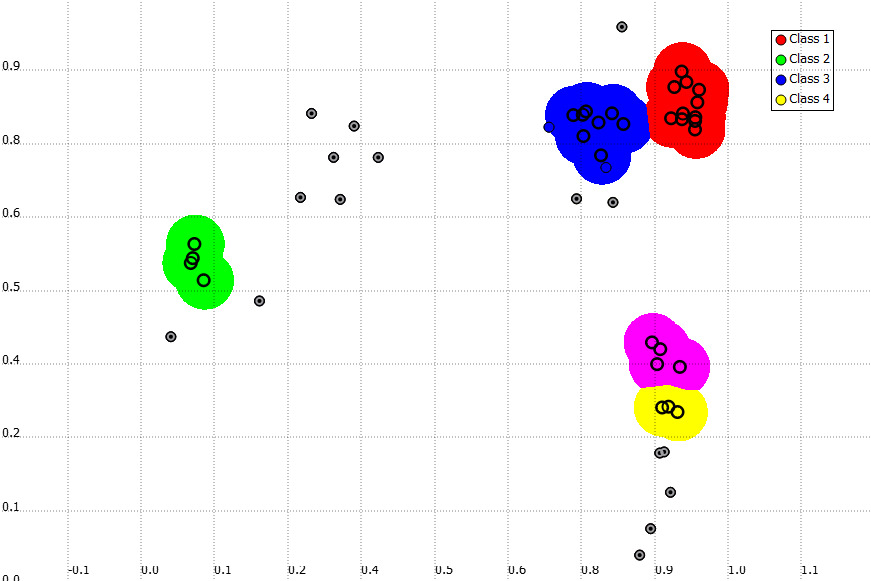
\includegraphics[width=\textwidth]{pictures/DBSCAN-Minpoint-2-epsilon005}
      \caption{$\epsilon = 0.05$}
      \label{fig:DBSCAN-Minpoint-2-epsilon005}
     \end{subfigure}
      ~
    \begin{subfigure}[t]{0.2\textwidth}
      \centering
      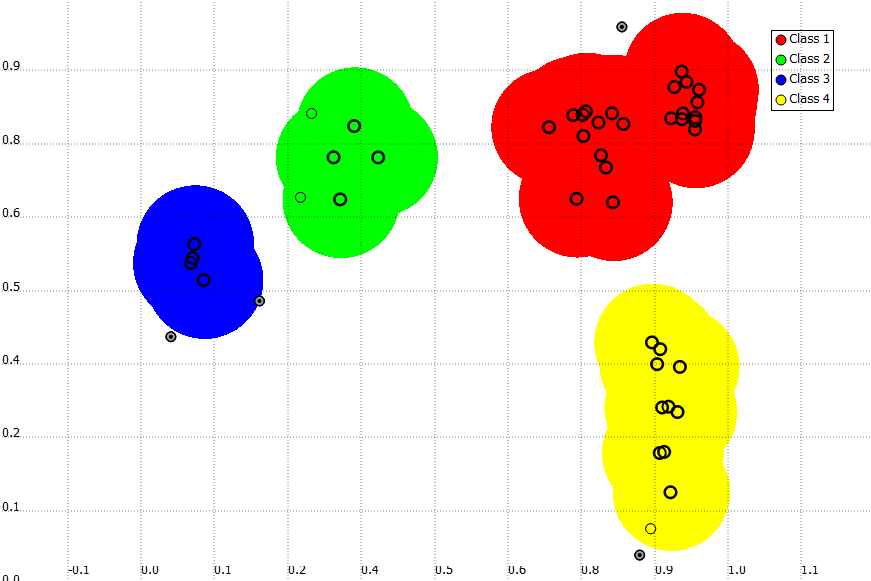
\includegraphics[width=\textwidth]{pictures/DBSCAN-Minpoint-2-epsilon01}
      \caption{$\epsilon = 0.1$}
      \label{fig:DBSCAN-Minpoint-2-epsilon01}
     \end{subfigure}
      ~
    \begin{subfigure}[t]{0.2\textwidth}
      \centering
      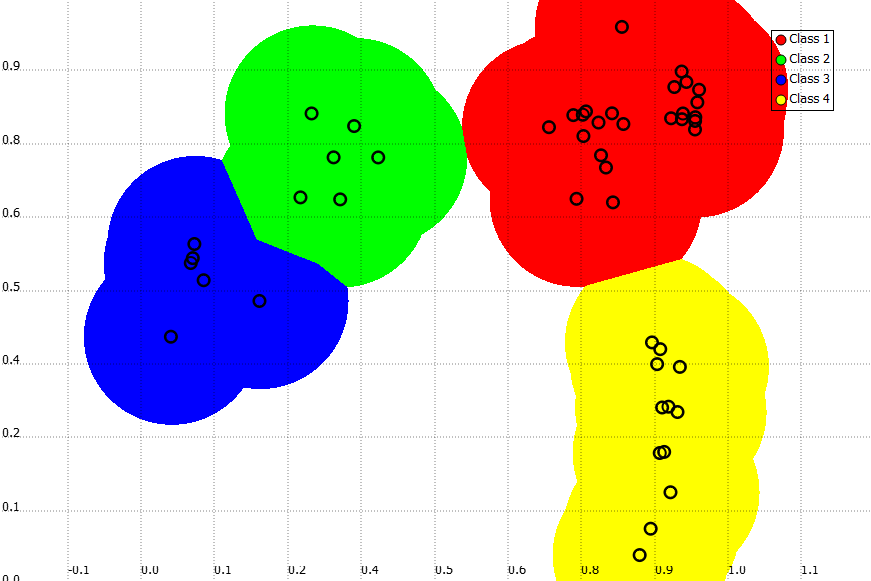
\includegraphics[width=\textwidth]{pictures/DBSCAN-Minpoint-2-epsilon015}
      \caption{$\epsilon = 0.15$}
      \label{fig:DBSCAN-Minpoint-2-epsilon15}
     \end{subfigure}
      ~
    \begin{subfigure}[t]{0.2\textwidth}
      \centering
      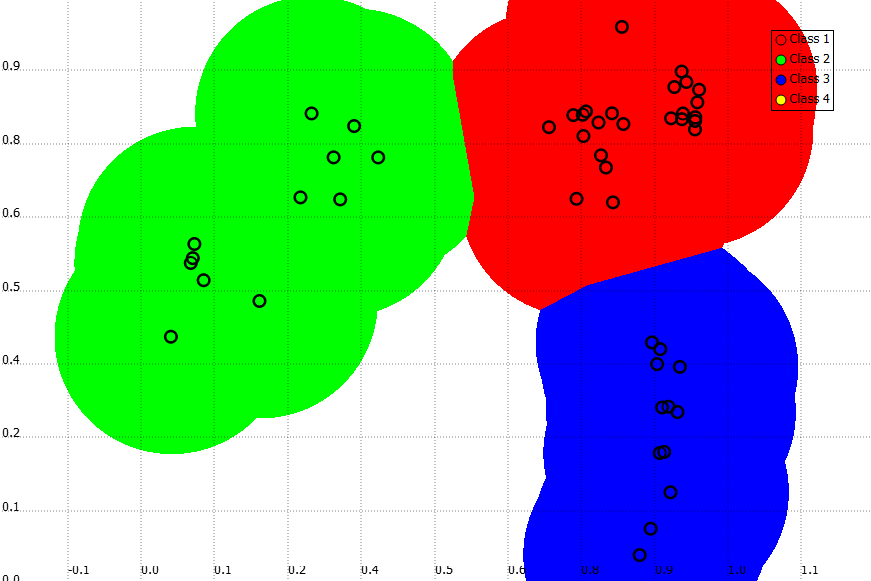
\includegraphics[width=\textwidth]{pictures/DBSCAN-Minpoint-2-epsilon02}
      \caption{$\epsilon = 0.2$}
      \label{fig:DBSCAN-Minpoint-2-epsilon02}
     \end{subfigure}
     \caption{Dataset 1 with DBSCAN clustering, $Minpoints = 2 $ and different value of $\epsilon$}
     \label{fig:DBScan_varyeps}
\end{figure}


% For K-Means and Soft-K-Means, you could report on the effect of the choice of the hyperparameters, metric and initialization on the position of the centroids, the shape of the regions, the found clusters, etc.

% For DBSCAN, it could refer to the number of clusters found with respect to the hyperparameters, the proportion of points considered as noise, etc.


\section{Classification - quantitative assessment}
% Report on performances when running the different classifiers.
% Report on values tested for i) the hyperparameters, ii) the training/testing ratios, iii) number of folds for crossvalidation. Give performance results only for the most interesting choices of hyperparameters, training/testing ratios and number of folds.

% \begin{wrapfigure}{r}{0.3\textwidth}
% 	\centering
% 	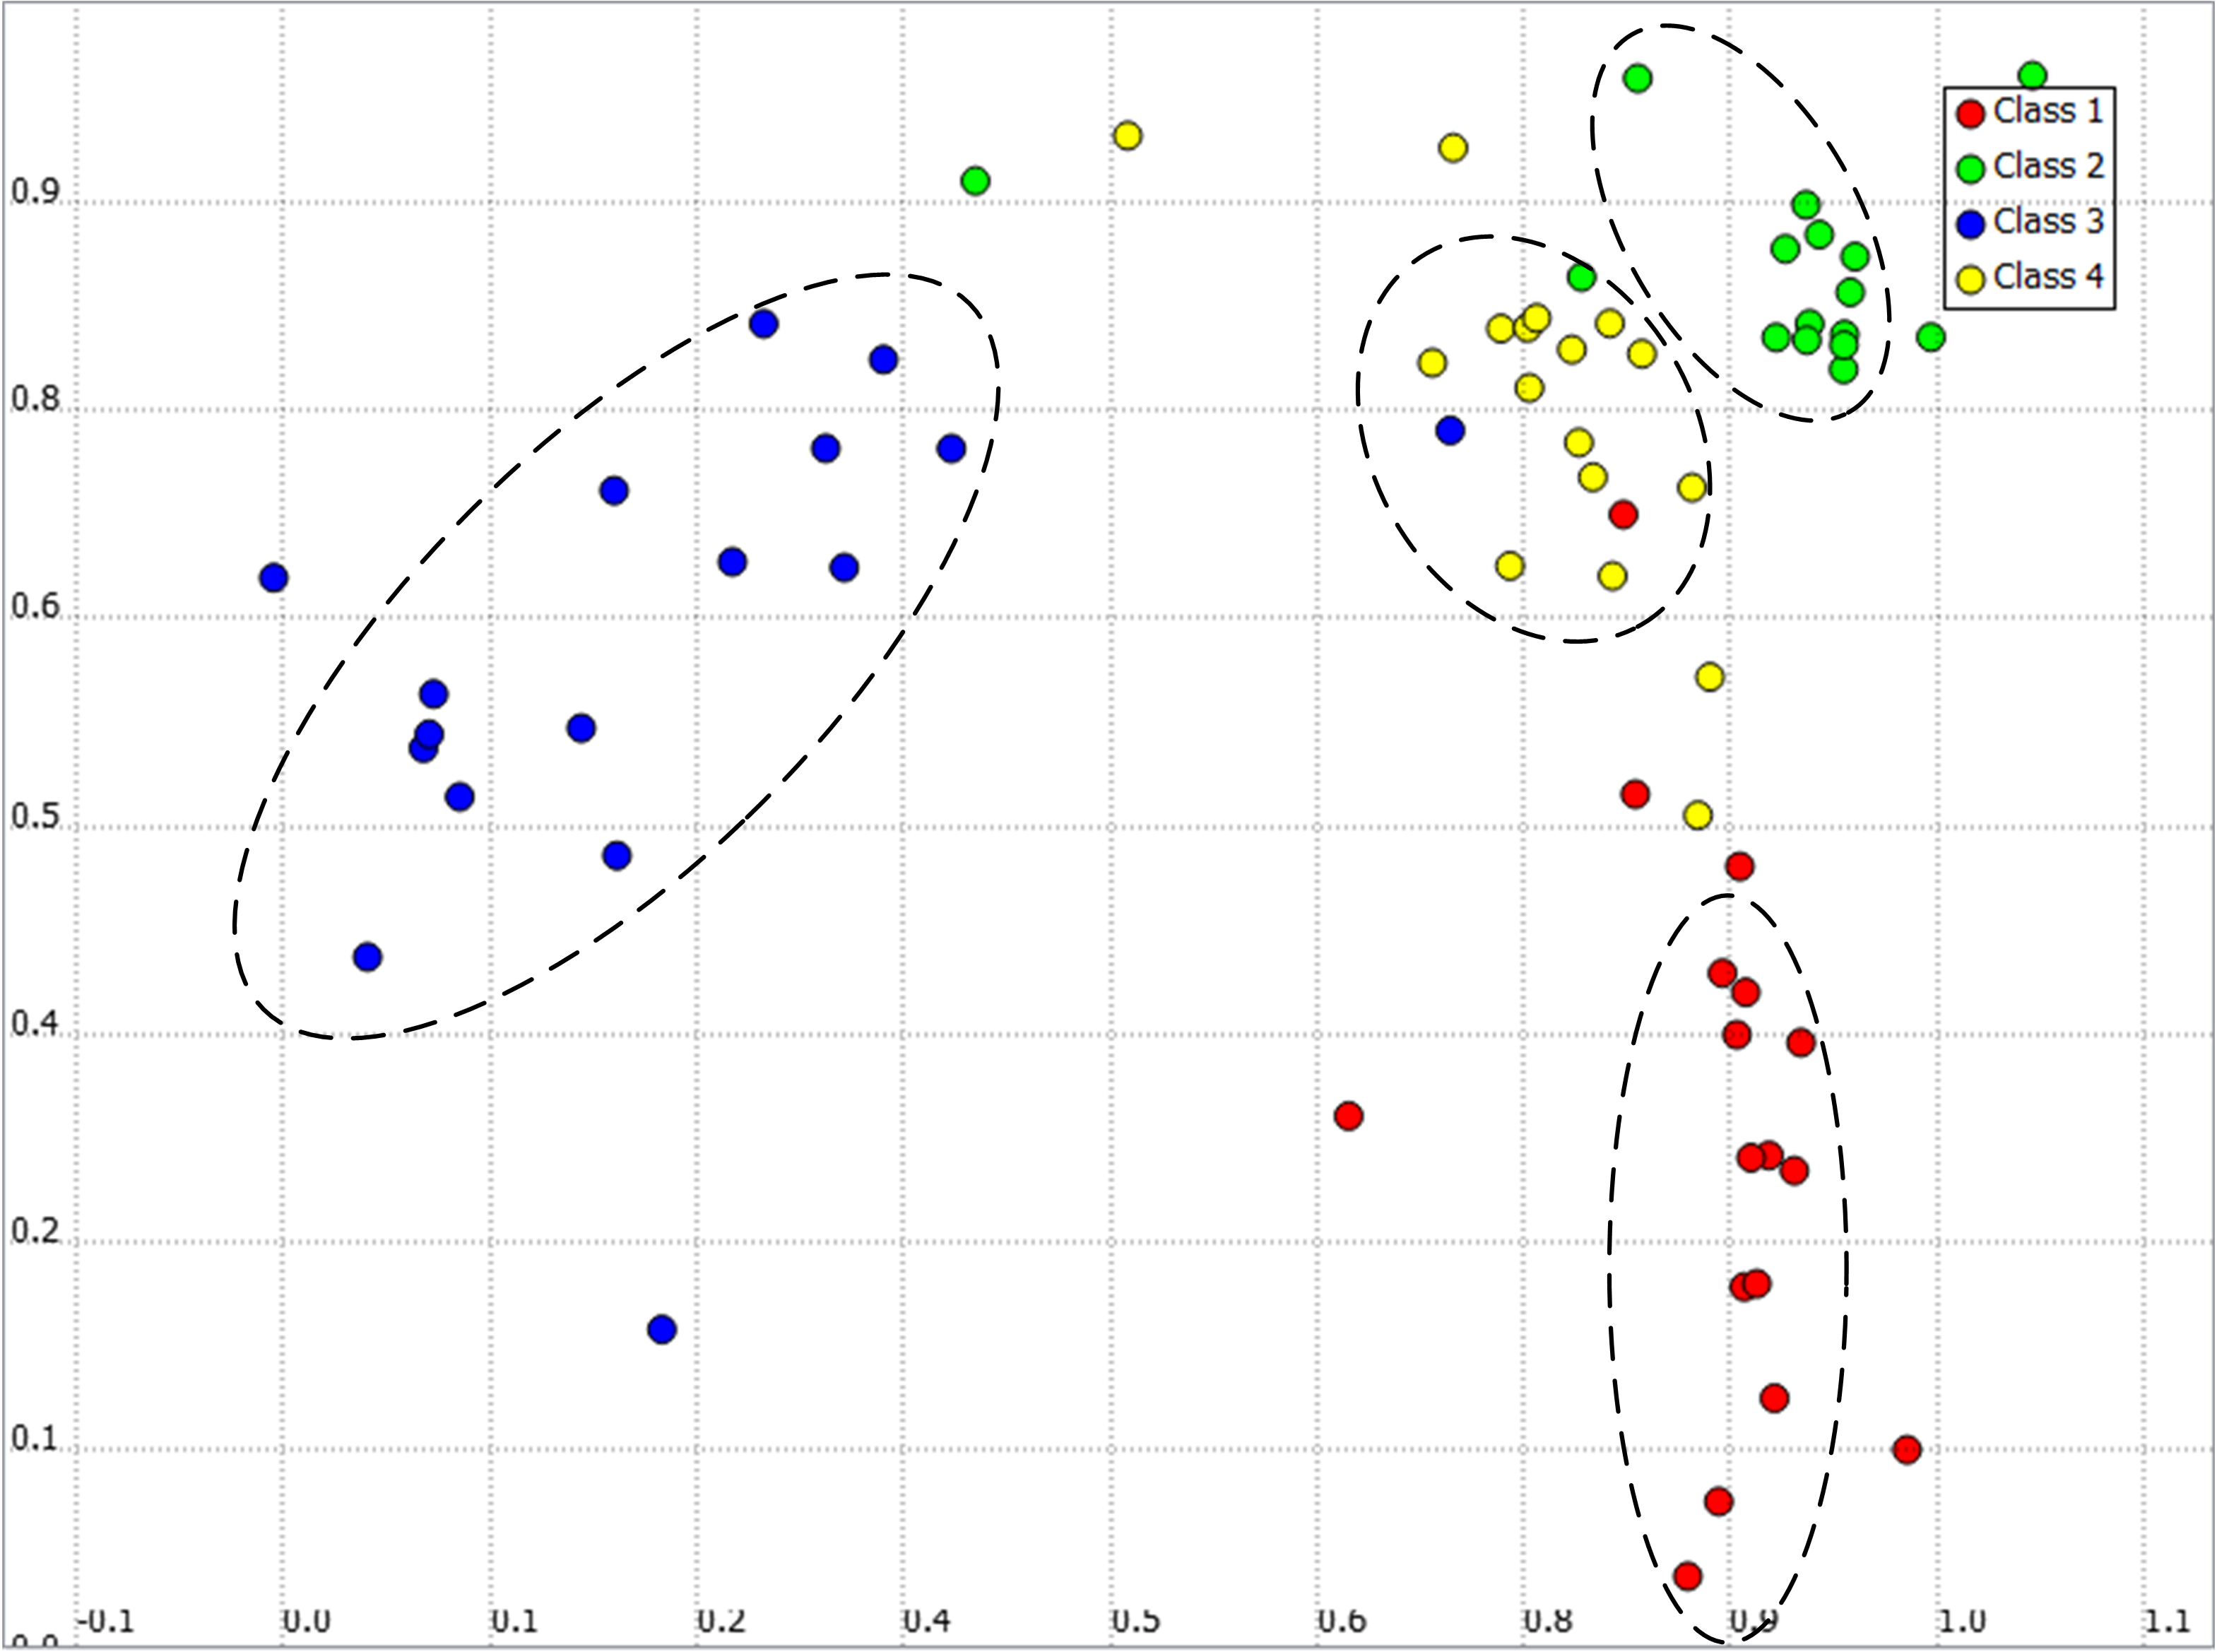
\includegraphics[width=0.25\textwidth]{pictures/dataset_new_2}
% 	\caption{Dataset 2}
%     \label{fig:dataset_new_2}
% \end{wrapfigure}
\subsection{Methods comparison}

The purpose of this section is to compare the GMM and SVM method with the dataset 2. Several factors can influence the performance of the GMM and C-SVM classification methods. Since there are many factors to take into account, a comparison plan is fixed in Figure \ref{fig:comparison-block-diag}. The first parameters to set are the test/ratio train and the number of folds for crossvalidation because these parameters directly influences the classification results for each method.


\begin{figure}[H]
	\centering
	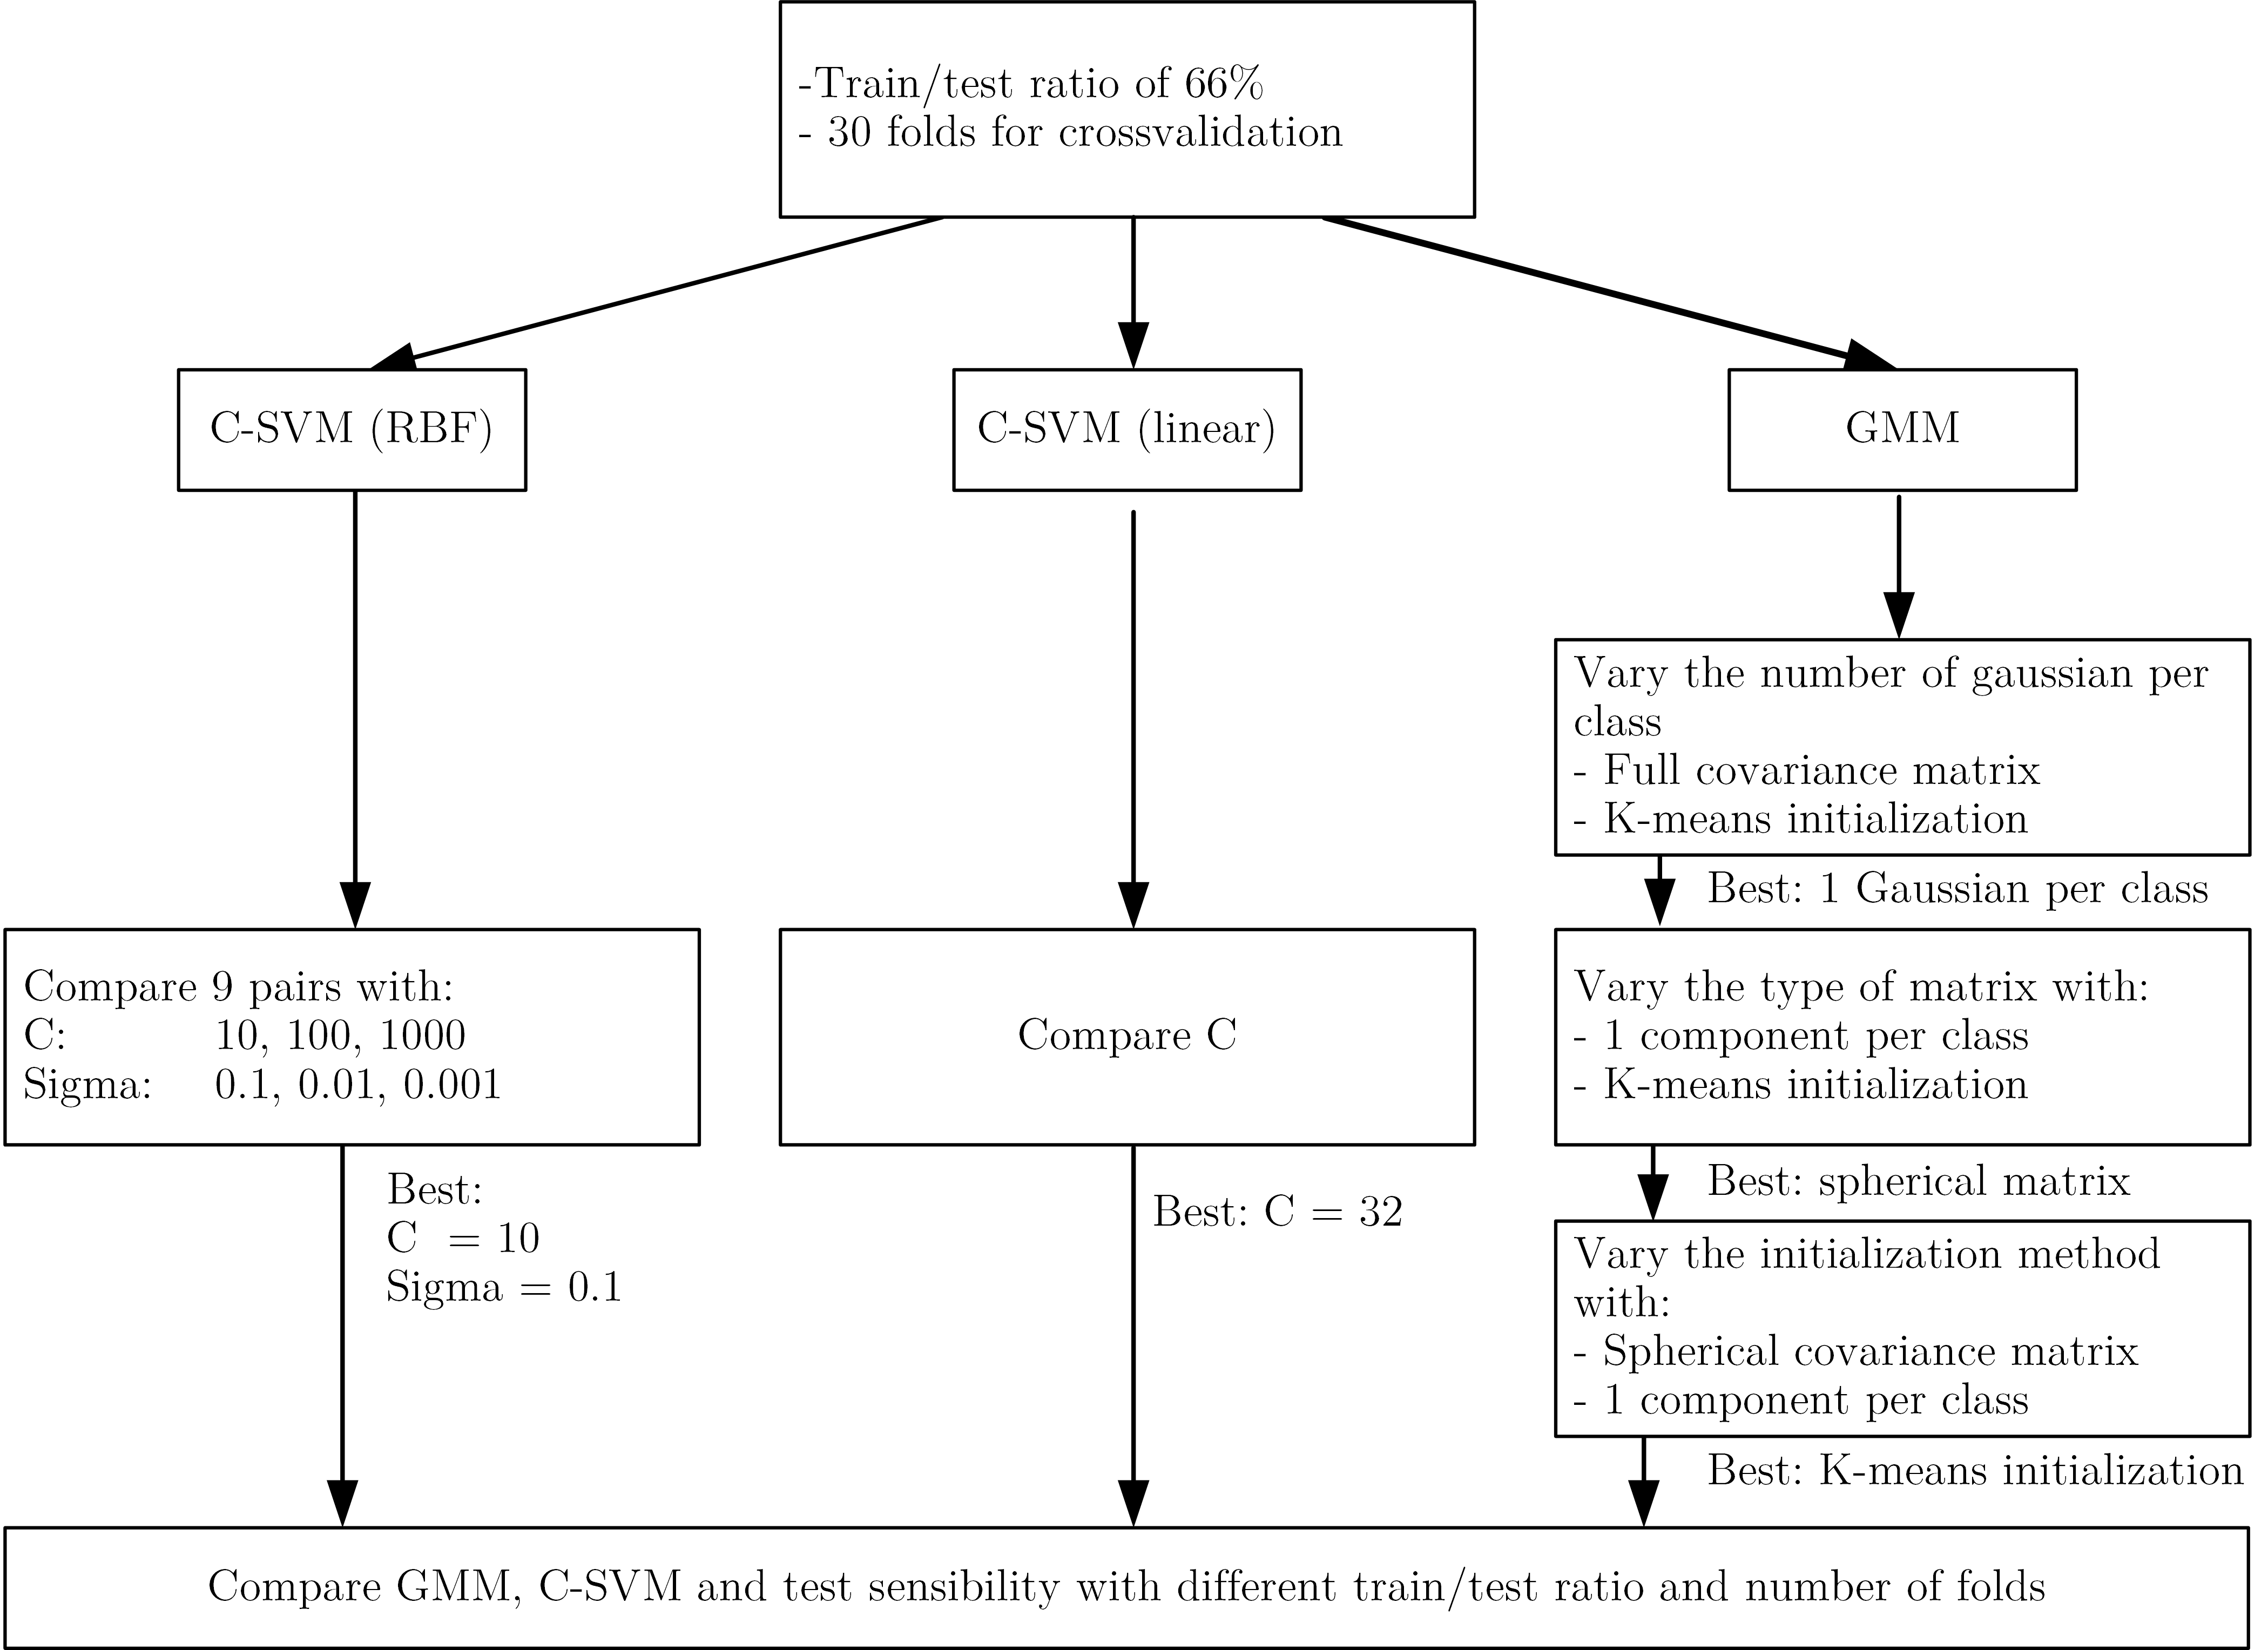
\includegraphics[width=0.7\textwidth]{pictures/comparison-block-diag}
	\caption{Comparison method block diagram}
	\label{fig:comparison-block-diag}
\end{figure}


\subsection{GMM classification}
For the GMM classification, the hyperparameters to be found were:

\begin{itemize}
  \item the number of gaussian components;
  \item the type of matrix (spherical, diagonal, full);
  \item the initialization method (random, uniform, K-Means).
\end{itemize}

 
 Quantitative analysis of classification methods are done with a train/test ratio of 66\% and 30 folds for crossvalidation. Further analysis on the choice of these two parameters is made in chapter \ref{fig:classifier_robustness}. Then, the hyperparameters were found in three stages. First, the K-Means initialization mode is set as it is a method expected to be more efficient than the random and uniform methods. A full covariance matrix is set to allow the algorith to chose each element of the covariance matrix and and therefore have as much freedom as possible. In Figure \ref{fig:GMM_graph_1} it is shown that the optimal choice for the number of gaussian components in this case would be 1.\\


\begin{figure}[H]
	\centering
	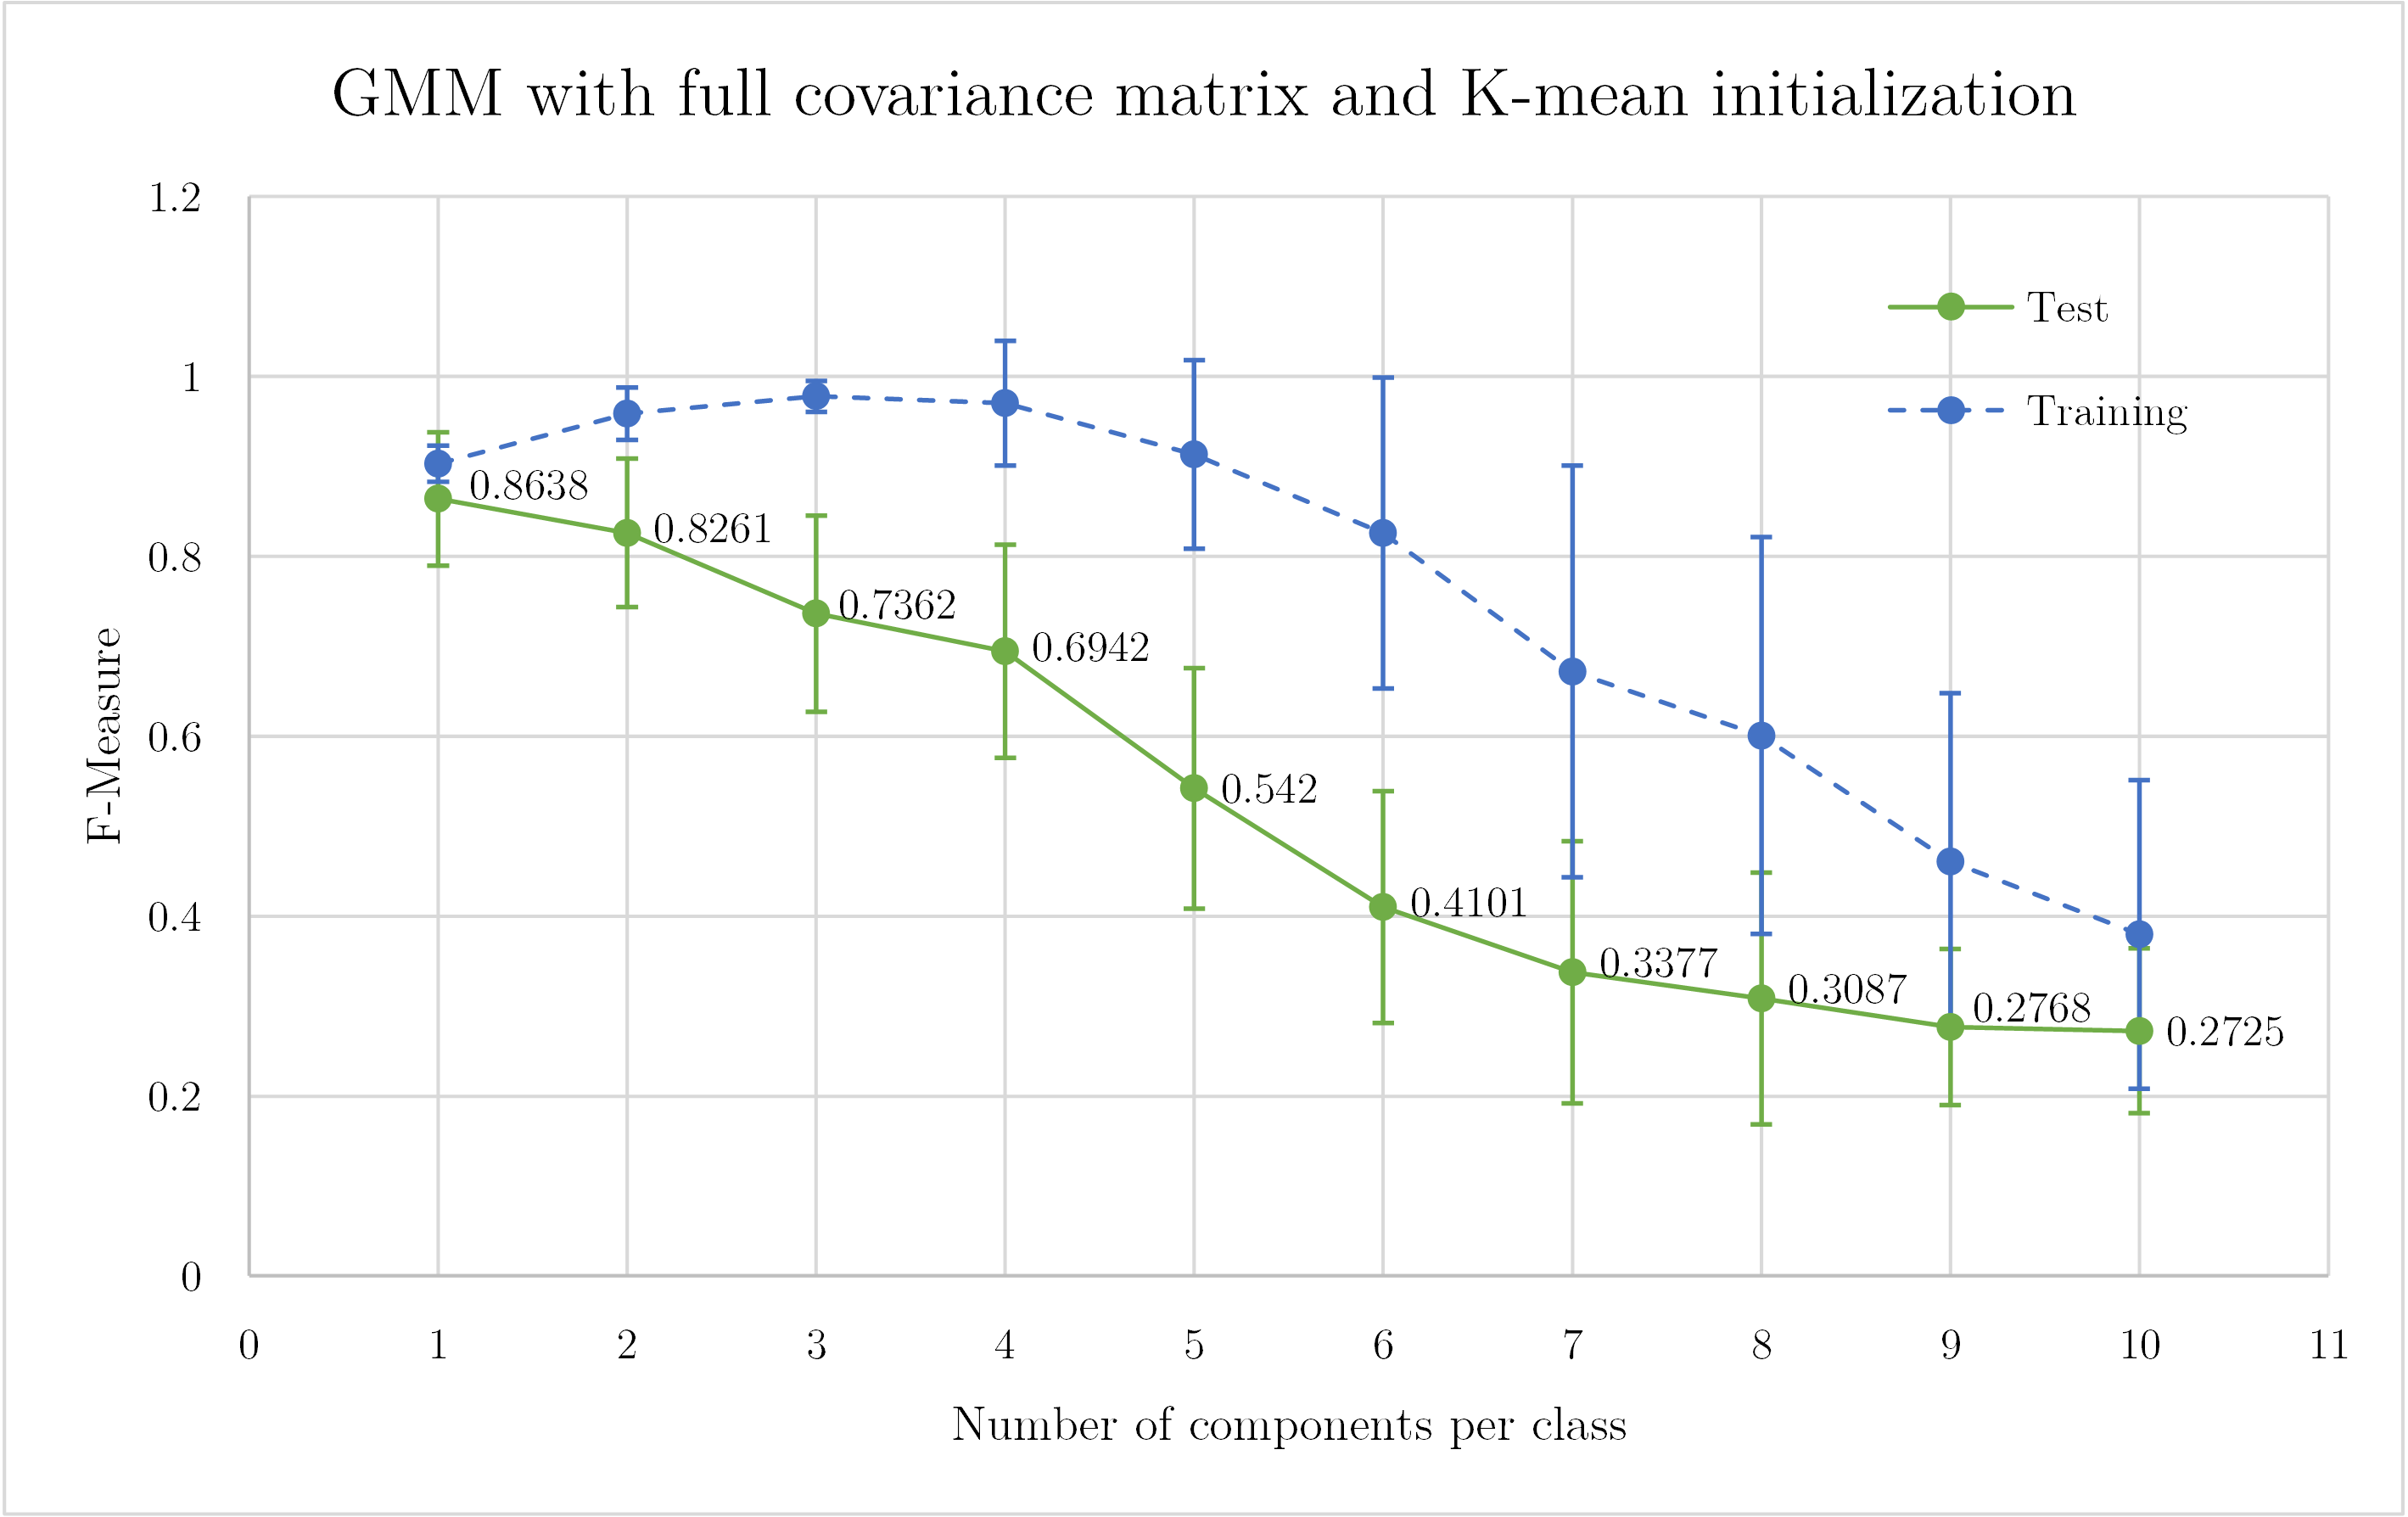
\includegraphics[width=0.5\textwidth]{pictures/GMM_graph_1}
	\caption{GMM: comparison for different number of gaussian components per class}
	\label{fig:GMM_graph_1}
\end{figure}

The training set shows better results with a higher number of GMMs per class but the F-Measure for the testing set gets worse and the variance becomes higher, which is possibly due to an overfitting phenomenon.
It can be noticed that for 4 and 5 components, the F-Measure's variance limit is higher than 1. As it is not possible to have a F-Measure higher than 1, this can be explained by the fact that the graph was produced with Excel, and the variance values are the same for the lower and higher limits.
TO REWRITE!!

\begin{figure}[H]
\centering
    \begin{subfigure}[t]{0.4\textwidth}
      \centering
      \includegraphics[width=0.9\textwidth]{pictures/GMM_graph_2}
      \caption{GMM: comparison for different type of matrix}
      \label{fig:GMM_graph_2}
     \end{subfigure}
      ~
    \begin{subfigure}[t]{0.4\textwidth}
      \centering
      \includegraphics[width=0.9\textwidth]{pictures/GMM_graph_3}
      \caption{GMM: comparison for different initialization}
      \label{fig:GMM_graph_3}
     \end{subfigure}
\caption{F-measure comparison for different type of matrix and initialization}
\label{fig:GMM_matrix_init}
\end{figure}

By following the procedure explained in the block diagram in Figure \ref{fig:comparison-block-diag}, the plots in Figure \ref{fig:GMM_matrix_init} are obtained. In particular, they show that a spherical covariance matrix and a K-Means initialization method achieve the smallest variance on the training set. Indeed, a large variance on the testing set indicates an overfitting problem of the training set.

\subsection{C-SVM classification (linear \& RBS)}

\begin{figure}[H]
\centering
    \begin{subfigure}[t]{0.45\textwidth}
      \centering
      \includegraphics[height=5cm]{pictures/linear-SVM}
      \caption{Linear C-SVM: comparison for different penalty factor C}
      \label{fig:linear-SVM}
     \end{subfigure}
      ~
    \begin{subfigure}[t]{0.45\textwidth}
      \centering
      \includegraphics[height=5cm]{pictures/non-linear-SVM}
      \caption{C-SVM with RBF kernel: comparison for different pairs of hyperparameters}
      \label{fig:non-linear-SVM}
     \end{subfigure}
     \caption{F-measure comparison for different type of matrix and initialization}
\end{figure}

The hyperparameter that must be choosen for the SVM classification method are:
\begin{itemize}
  \item the penalty term C;
  \item the width of the RBS kernel (RBS only).
\end{itemize}

 For the linear SVM, the C parameter was trained and tested for values going from 1 to 4096, 32 by 32. In Figure \ref{fig:linear-SVM} it can be observed that the highest F-measure average for the testing set corresponds to $C=16$, but in order to have a lower testing variance a $C = 32$ was chosen. Lower variance is preferable to minimize the overfitting of the training set even though the average of the F-Measure is slightly smaller.\\

 For the non-linear SVM classification, values of $\sigma$ and C are chosen as specified in Figure \ref{fig:comparison-block-diag} and all combinations are compared in Figure \ref{fig:non-linear-SVM}, which shows that the combination that optimizes the testing F-Measure is $ C = 10 $ and $ \sigma = 0.1$ with the highest F-measure and the lowest variance. Indeed, it can be noticed that, for each chosen C, the testing F-Measure degrades and its variance increases as the $\sigma$ decreases , while the training F-Measure increases and its variance decreases. This can be explained by a overfitting phenomenon. 


 \begin{figure}[H]
\centering
    \begin{subfigure}[t]{0.3\textwidth}
      \centering
      \includegraphics[height=5cm]{pictures/non-linear-SVM_fixeRBF}
      \caption{C-SVM with RBF kernel: comparison for different penalty factor C  and $\sigma = 0.1$}
      \label{fig:non-linear-SVM_fixeRBF}
     \end{subfigure}
      ~
    \begin{subfigure}[t]{0.3\textwidth}
      \centering
      \includegraphics[height=5cm]{pictures/non-linear-SVM_fixeC}
      \caption{C-SVM with RBF kernel: comparison for different width $\sigma$ and a penalty factor $C = 1$}
      \label{fig:non-linear-SVM_fixeC}
     \end{subfigure}
     \caption{F-measure comparison for different type of matrix and initialization}
\end{figure}

\subsection{C-SVM and GMM comparison}

The SVM method with an RBF kernel is the most appropriate for classifying dataset 2.\\
\todo{Expliquer un peu plus}

\begin{figure}[H]
\centering
	\begin{subfigure}[t]{0.3\textwidth} \label{fig:best-GMM}
      \centering
      \includegraphics[height=3.2 cm]{pictures/Compare-best-classification-training}
      \caption{Training set}
      \label{fig:Compare-best-classification-training}
    \end{subfigure}%
    ~
    \begin{subfigure}[t]{0.3\textwidth} \label{fig:best-SVM}
      \centering
      \includegraphics[height=3.2 cm]{pictures/Compare-best-classification-test}
      \caption{Test set}
      \label{fig:Compare-best-classification-training}
     \end{subfigure}
      ~
    \begin{subfigure}[t]{0.3\textwidth} \label{fig:best-C-SVM}
      \centering
      \includegraphics[height= 3.2 cm]{pictures/classification-best.png}
      \caption{C-SVM ($\sigma = 0.1$ and $C=10$)}
      \label{fig:classification-best}
     \end{subfigure}
      ~
     \caption{F-measure box-plot comparison with a train/test ratio of 66\% and 30 folds for cross validation.}
\end{figure}


\subsection{Classifiers robustness} \label{fig:classifier_robustness}

\begin{figure}[H]
\centering
	\begin{subfigure}[t]{0.3\textwidth} \label{fig:best-GMM}
      \centering
      \includegraphics[height=3.2 cm]{pictures/train-test-ratio-low-10percent-train-data}
      \caption{Training set}
      \label{fig:train-test-ratio-low-10percent-train-data}
    \end{subfigure}%
    ~
    \begin{subfigure}[t]{0.3\textwidth} \label{fig:best-SVM}
      \centering
      \includegraphics[height=3.2 cm]{pictures/train-test-ratio-low-10percent-test-data}
      \caption{Testing set}
      \label{fig:train-test-ratio-low-10percent-train-data}
     \end{subfigure}
      ~
     \caption{F-measure box-plot comparison with a train/test ratio of 66\% and 30 folds for cross validation.}
\end{figure}

\textbf{Train/test ratio}\\
As the dataset in question is quite small, the training/testing ratio must be carefully chosen. Indeed, the lower the ratio, the less the classifier will be trained but the more it will be robust (less variance on testing set). This is a good approach for a dataset with enough datapoints. On the contrary, the higher the ratio, the more the classifier will be possibly overfitting to the training set and the variance for unseen data will be higher. A good trade-off was found to be the ratio $0.667$.

ADD PROOF!!

\textbf{Number of folds sensitivity}\\
In MLDemos, the crossvalidation method is based on a random separation of the data between train and test on which the classifier is applied. The separation is then repeated f times and the results in the end are averaged. With this type of crossvalidation a sufficiently large number of folds is recommended to obtain consistent results with lower variance. However, a too high number of repetitions is not useful because after a while the results do not improve but the cost of calculation increases. A good trade-off for our dataset was found to be 30 folds as it was at this point that the results started to stabilize between several cross validation process.

ADD PROOF!!

\subsection{Overall discussion and conclusion}

% Offer an overall appraisal of your work and draw conclusions about the results achieved.

\end{document}